
\documentclass{template/openetcs_report}
% Use the option "nocc" if the document is not licensed under Creative Commons
%\documentclass[nocc]{template/openetcs_article} 
\usepackage{xspace}
\usepackage{graphicx}
\usepackage[final,nomargin,inline]{fixme}
\usepackage{lscape} 
\usepackage{listings}
\usepackage{placeins}
\usepackage{framed}
\usepackage{booktabs}
\usepackage{amsmath}
\usepackage{amssymb}
\usepackage{stmaryrd}
\usepackage{dashbox}
\usepackage[pdftex]{hyperref}

\usepackage{multirow}
\usepackage{multicol}

\numberwithin{figure}{chapter}
\numberwithin{table}{chapter}
\usepackage{float}
\floatstyle{plain}
\newfloat{listing}{thp}{lop1}[chapter]
\floatname{listing}{Listing}

\renewcommand\floatpagefraction{.90}
\renewcommand\topfraction{.90}
\renewcommand\bottomfraction{.90}
\renewcommand\textfraction{.10}
\setlength{\unitlength}{1mm}


%user specified macros


\newcommand{\VV}{Verification \& Validation\xspace}
\newcommand{\vv}{verification \& validation\xspace}

\def\CC{{C\nolinebreak[4]\hspace{-.05em}\raisebox{.4ex}{\tiny\bf ++}}}

\newcommand{\adhesion}{\mbox{\inl{AdhesionFactor}}\xspace}

\newcommand{\bitwalker}{\mbox{\texttt{Bitwalker}}\xspace}

\newcommand{\poke}{\mbox{\texttt{Bitwalker\_Poke}}\xspace}
\newcommand{\peek}{\mbox{\texttt{Bitwalker\_Peek}}\xspace}
\newcommand{\acsl}{\mbox{\textsf{ACSL}}\xspace}
\newcommand{\isoc}{\mbox{\textsf{C}}\xspace}
\newcommand{\framac}{\mbox{\textsf{Frama-C}}\xspace}
\newcommand{\framacwp}{\mbox{\textsf{Frama-C\slash WP}}\xspace}
\newcommand{\why}{\mbox{\textsf{Why}}\xspace}
\newcommand{\wpframac}{\mbox{\textsf{WP}}\xspace}
\newcommand{\altergo}{\mbox{\textsf{Alt-Ergo}}\xspace}
\newcommand{\qed}{\mbox{\textsf{Qed}}\xspace}
\newcommand{\cvc}{\mbox{\textsf{CVC4}}\xspace}
\newcommand{\z}{\mbox{\textsf{Z3}}\xspace}
\newcommand{\coq}{\mbox{\textsf{Coq}}\xspace}
\newcommand{\cealist}{\mbox{\textsf{CEA LIST}}\xspace}
\newcommand{\fokus}{\mbox{\textsf{Fraunhofer FOKUS}}\xspace}

\newcommand{\inl}[1]{\lstinline[style=inline]{#1}}


%Defining C-Code Environment

\usepackage{courier} 
\usepackage{listings}
\usepackage{color} 

% fix bug with listing under texlive-2014
% see https://lists.debian.org/debian-tex-maint/2014/06/msg00209.html

\makeatletter
\renewcommand\lstinline[1][]{%
  \leavevmode\bgroup % \hbox\bgroup --> \bgroup
  \def\lst@boxpos{b}%
  \lsthk@PreSet\lstset{flexiblecolumns,#1}%
  \lsthk@TextStyle
  \ifnum\iffalse{\fi`}=\z@\fi
  \@ifnextchar\bgroup{%
  \ifnum`{=\z@}\fi%
  \afterassignment\lst@InlineG \let\@let@token}{%
  \ifnum`{=\z@}\fi\lstinline@}}
\makeatother


%\definecolor{darkred}		{rgb}{0.60,0.00,0.00}
\definecolor{coACSLBehavior}	{rgb}{0.30,0.00,0.00}
\definecolor{coASCL}		{rgb}{0.00,0.10,0.00}
\definecolor{coASCLKeyword}	{rgb}{0.00,0.10,0.10}
\definecolor{darkgreen}		{rgb}{0.00,0.40,0.00}
%\definecolor{red}		{rgb}{0.98,0.00,0.00}
\definecolor{darkblue}		{rgb}{0.00,0.00,0.60}
%\definecolor{lightblue}		{rgb}{0.60,0.80,1.00}
%\definecolor{lightred}		{rgb}{1.00,0.60,0.60}
\definecolor{coCKeyword}	{rgb}{0.00,0.00,0.60}

\lstdefinestyle{acsl-block}
{	emph=[1]{assert, assumes, assigns, axiom, axiomatic, decreases, ensures,
                 ghost, invariant, lemma, logic, loop, predicate,
		 reads, requires, variant},
	emphstyle=[1]{\bfseries\color{coASCLKeyword}},
	emph=[2]{behavior, behaviors, complete, disjoint, for:},
	emphstyle=[2]{\bfseries\color{coACSLBehavior}},
	emph=[3]{typedef, int, char, integer, real, bool, size_type, value_type, uint8_t,  uint64_t},
	emphstyle=[3]{\bfseries\color{coCKeyword}},
	escapeinside={//`}{`//},
	morecomment=*[l][\color{coASCL}]{//@},
	morecomment=*[s][\color{coASCL}]{/*@}{*/},
	moredelim=*[is][\bfseries]{|*}{*|},
	%emphstyle=[3]{\ttfamily}
	}

\lstdefinestyle{func-decl}
{	emph=[1]{assert, assumes, assigns, axiom, axiomatic, decreases, ensures,
                 ghost, invariant, lemma, logic, loop, predicate,
		 reads, requires, variant},
	emphstyle=[1]{\bfseries\color{coASCLKeyword}},
	emph=[2]{behavior, behaviors, complete, disjoint, for:},
	emphstyle=[2]{\bfseries\color{coACSLBehavior}},
	emph=[3]{integer, real, size_type, value_type},
	emphstyle=[3]{\bfseries\color{coCKeyword}},
	escapeinside={//`}{`//},
	morecomment=*[l][\color{coASCL}]{//@},
	morecomment=*[s][\color{coASCL}]{/*@}{*/},
	moredelim=*[is][\bfseries]{|*}{*|},
    frame=none,
    numbers=none
	%emphstyle=[3]{\ttfamily}
	}

\lstdefinestyle{acsl-inline}
{	emph=[1]{assert,assigns, assumes, axiom, axiomatic, decreases, ensures, ghost, invariant, lemma, logic, loop,
             predicate, reads, requires, return, variant },
	emphstyle=[1]{\bfseries\color{coASCLKeyword}},
	emph=[2]{behavior, behaviors, complete, disjoint, for:},
	emphstyle=[2]{\bfseries\color{coACSLBehavior}},
	emph=[3]{typedef, int, char, integer, real, bool, size_type, value_type, uint8_t,  uint64_t},
	emphstyle=[3]{\bfseries\color{coCKeyword}},
	morecomment=*[l][\color{coASCL}]{//@},
	morecomment=*[s][\color{coASCL}]{/*@}{*/},
	moredelim=*[is][\bfseries]{|*}{*|}
}

\lstdefinestyle{inline}
{      % basicstyle = \ttfamily\small\color{coASCL},
	keywordstyle = \ttfamily\normal\color{coASCL},
	stringstyle=\color{coASCL},
	style=acsl-inline,
	breaklines= false
}

\lstset{%
  language=C++,
  defaultdialect=ansi,
  basicstyle=\footnotesize\ttfamily,
  commentstyle=\small\color{darkgreen},
  keywordstyle=\small\bfseries\color{darkblue},
  stringstyle=\small\color{darkgreen},
  tabsize = 2,
  showspaces=false,
  showtabs=false,
  columns=fixed,  
  frame=none,  
  breaklines=true,
  showstringspaces=false,
  xleftmargin=0.2cm,
  %rangeprefix=//label, % to specify a certain range from a file
  %rangesuffix=;, % to be shown
  %includerangemarker=false,
	numbers=none
}


\graphicspath{{./template/}{.}{./images/}}
\begin{document}
\frontmatter
\project{openETCS}

%Please do not change anything above this line
%============================
% The document metadata is defined below

%assign a report number here
\reportnum{OETCS/WP4/D4.3.2}

%define your workpackage here
\wp{Work Package 4: ``Validation \& Verification Strategy''}

%set a title here
\title{Final Report on Validation and Verification Report of Implementation/Code}

%set a subtitle here
%\subtitle{Description of Work}

%set the date of the report here
\date{December 2015}

%define a list of authors and their affiliation here

\creatorname{Jens Gerlach}
\creatoraffil{Fraunhofer FOKUS}

\techassessorname{Virgile Prevosto}
\techassessoraffil{CEA LIST}

\qualityassessorname{Abdelnasir Mohamed}
\qualityassessoraffil{AEbt}

\approvalname{Klaus-R\"udiger Hase}
\approvalaffil{DB Netz}

\author{J.\ Gerlach, J.\ Burghardt, T.\ Lapawczyk}
\affiliation{Fraunhofer FOKUS\\
  Kaiserin-Augusta-Allee 31 \\
  10589 Berlin, Germany\\
  jens.gerlach@fokus.fraunhofer.de \\
  www.fokus.fraunhofer.de}

\author{M.\ Behrens}
\affiliation{DLR Institute of Transportation Systems\\
Lilienthalplatz 7\\
Braunschweig 38108, Germany\\
www.dlr.de/ts}


% define the coverart
\coverart[width=350pt]{openETCS_EUPL}

%define the type of report
\reporttype{Intermediate report}

\sloppy % nicht schön, aber selten!-)

\begin{abstract}
  This work package will comprise the activities concerned with
  verification and validation within openETCS. This includes \vv of
  development artifacts, that is, showing that models and code
  produced correctly express or implement what they are supposed
  to. And also, methods and tools to perform such tasks will be
  evaluated with the goal of assembling a suitable method and tool
  chain to support a full development.
\end{abstract}

%=============================
%Do not change the next three lines
\maketitle
\tableofcontents
\listoffiguresandtables
\clearpage
\listof{listing}{List of code examples}
%\listoffixmes
\cleardoublepage
%=============================

% The actual document starts below this line
%=============================

\mainmatter
%Start here

\section{Introduction}\label{sec:intro}
% ==========================================================================

\subsection{A Test Model for the ETCS Ceiling Speed Monitor}
In 2011 the {\it model-based testing benchmarks website} www.mbt-benchmarks.org has been 
created with the objective to publish test models that may serve as challenges or benchmarks 
for validating testing theories   and for comparing the capabilities of model-based testing (MBT) tools~\cite{pel2011a}.
In this technical report a novel contribution to this website is presented, a SysML model
of the Ceiling Speed Monitor (CSM) which is part of the European Vital Computer (EVC), the onboard controller of trains conforming to the European Train Control System (ETCS) standard~\cite{ETCS}. In    Section~\ref{sec:ceil} the functional objectives for the CSM are described, and in Section~\ref{sec:modeldesc} the detailed model description is provided. 

The static and behavioural semantics of SysML models have been defined in~\cite{SysML12,uml_2_4} in a semi-formal way, leaving certain ``semantic variation points'' open, so that they can be adjusted according to project-specific requirements. For automated model-based testing, however, a strictly formal semantics is required, so that concrete test data can be calculated from the model's transition relation using constraint solving techniques~\cite{peleska2013ictss}. 
We therefore describe in Section~\ref{sec:transrel} how a formal behavioural semantics is derived for the CSM model and present the associated transition relation in propositional form.

We use state transition systems (STS) for encoding the operational semantics of concrete
modelling formalisms like SysML. STS are widely known from the field of model checking~\cite{clarke_em-etal:1999a}, because their extension into Kripke Structures allows for effective data abstraction techniques. The latter are also applied for equivalence class testing. 
Since state transition systems are a means for semantic representation, testing theories elaborated for STS are applicable for all concrete formalisms whose behavioural semantics can be expressed by STS. In~\cite{d341} it is shown how the semantics of general SysML models and models of a process algebra are encoded as STS. In this technical report we illustrate  how this is achieved for the concrete case of the CSM SysML model.

% ==========================================================================
\subsection{Equivalence Class Partition Testing for the CSM}

The CSM represents a specific test-related challenge: its behaviour depends on actual and allowed speed, and these have conceptually real-valued data domains, so that -- even when   discretising
the input space -- it would be infeasible to exercise all possible combinations of 
inputs on the system under test (SUT). Therefore equivalence class partition (ECP)
 testing strategies have 
to be applied for testing the CSM. While these strategies are well-adopted  in a heuristic manner
in today's industrial test campaigns, practical application of equivalence class testing still lacks 
formal justification of the equivalence classes selected and the sequences of class representatives 
selected as test cases: standard text books used in industry, for example~\cite{spillner2006}, 
only explain the generation of input equivalence class tests for   systems, where the 
SUT reaction to an input class representative is independent on the internal state. Moreover, the systematic calculation of classes from models, as well as their formal justification with respect to
test strength and coverage achieved, is not yet part of today's best practices in industry. 

In contrast to this, formal approaches to equivalence class testing have been studied in the formal methods communities; references to these results  are given in Section~\ref{sec:related}.
In the second main part of this report (Section~\ref{sec:iecpstart}) we therefore describe a recent formal technique for equivalence class testing and its application to testing the CSM. The theoretical 
foundations of this strategy have been published by two of the authors in~\cite{peleska2013ictss}. 
This technical report illustrates its practical application and presents first evaluation details using a 
prototype implementation in an existing MBT tool; the ECP tests are  compared to test results obtained when applying other MBT coverage strategies, such as transition cover or MC/DC coverage (Section~\ref{sec:conventionaltests}). 


% ==========================================================================
\subsection{Fault Models and Completeness Results}


Our ECP strategy
introduces test suites depending on {\it fault models}. This well adopted notion has first been 
introduced in the field of finite state machine (FSM) testing~\cite{petrenko1996}, but is also applicable
to other formal modelling techniques. A fault model consists of a reference model, a conformance relation and a fault domain. The latter is a collection of models whose behaviour may or may not be
consistent to the reference model in the sense of the conformance relation. The test suites generated 
by the ECP strategy described here are {\it complete} with respect to the given fault model: each
system of the fault domain which conforms to the reference model will pass all the generated tests
(this means that the test suite is {\it sound}), and each system in the fault domain that violates the
conformity to the reference model will fail at least  once when tested according to the test suite (the test suite is {\it exhaustive}). 




%%% @todo open proof strategy of the openETCS project




\cleardoublepage

\chapter{An introduction to formal verification with \framacwp}
\label{sec:frama-c}

Frama-C is a platform dedicated to source-code analysis of C software.
It has a plug-in architecture and can thus be easily extended to 
different kinds of analyses.
The WP plugin of Frama-C allows one to formally verify that a piece of
C code satisfies its specification.
This implies, of course, that the user provides a \emph{formal specification}
of what the implementation is supposed to do.
Frama-C comes with its own specification language ACSL which stands for
\emph{ANSI\slash ISO C Specification Language}.
In order to help potential users to master ACSL we discuss in this chapter 
a very simple C function \inl{abs_int} that implements the computation of
the absolute value for objects of type~\inl{int}.

\begin{itemize}
\item
In Section~\ref{sec:first-steps} we will present a straightforward
specification of \inl{abs_int}.
We discuss the reasons why \framacwp is not able to verify that our
implementation satisfies this specification in Section~\ref{sec:framac-failure}.

\item 
In Section~\ref{sec:contract-sharpening} we provide a more precise
specification that can be verified by \framacwp.
In Section~\ref{sec:separating-spec-impl} we explain
how \framac supports---by allowing the separation of the specification from the 
implementation---good software engineering practices.

\item
Sections~\ref{sec:modular-verification} and~\ref{sec:side-effects}
discuss, respectively,
how \framacwp supports \emph{modular verification} and the
formal treatment of \emph{side effects}.
\end{itemize}

\clearpage

\section{First steps}
\label{sec:first-steps}

We will consider the function that computes the absolute value $|x|$
of an integer $x$.
In order to avoid name clashes with the function \inl{abs} in C standard library
we use the name \inl{abs_int}.

The mathematical definition of absolute value is very simple
\begin{align}
\label{eq:abs}
   |x| &= \left\{
            \begin{array}{rl}
               x  & \text{if $x \geq 0$} \\
               -x & \text{if $x < 0$}
            \end{array}
          \right.
\end{align}

A straightforward implementation of \inl{abs_int} is shown in Listing~\ref{lst:abs}.

\begin{listing}[hbt]
\begin{minipage}{\textwidth}
\lstinputlisting[style=acsl-block ]{./Abs/abs.c}
\end{minipage}
\caption{\label{lst:abs} An implementation of the absolute value function}
\end{listing}

In order to demonstrate that this implementation is correct we have to provide
a formal specification.
Listing~\ref{lst:abs1} shows our first attempt for an ACSL specification of \inl{abs_int} that
is based on the mathematical definition of the function $x \mapsto |x|$ in Equation~\ref{eq:abs}.

\begin{listing}[hbt]
\begin{minipage}{\textwidth}
\lstinputlisting[style=acsl-block ]{./Abs/abs1.c}
\end{minipage}
\caption{\label{lst:abs1} A first attempt to formally specify \inl{abs_int}}
\end{listing}

\FloatBarrier

The first thing to note is that ACSL specifications---or \emph{contracts}---are placed in special C comments
(they start with \inl{/*@}).
Thus, they do not interfere with the executable code.
The \inl{ensures} clause in the specification expresses \emph{postconditions},
that is, properties that should be guaranteed \emph{after} the execution
of \inl{abs_int}.
The ACSL reserved word \inl{\\result} is used to refer to the return value of a C function.
Note that we use the usual C operators \inl{==} and \inl{<=} to express equalities and inequalities
in the specification.
There is also an additional operator \inl{==>} which expresses logical implication.

\section{Why can \framacwp not verify such a simple function?}
\label{sec:framac-failure}

Although the specification and implementation in Listing~\ref{lst:abs1} look perfectly right, 
\framacwp cannot verify that the implementation actually satisfies its specification.


The reason becomes clear if we look at some actual return values of \inl{abs_int}.
Listing~\ref{lst:test_abs} shows our test code whose output is
listed in Table~\ref{tbl:test_abs_output}.

\begin{listing}[hbt]
\begin{minipage}{\textwidth}
\lstinputlisting[style=acsl-block ]{./Abs/test_abs.c}
\end{minipage}
\caption{\label{lst:test_abs} Some simple test cases for \inl{abs_int}}
\end{listing}

%\clearpage

\begin{table}[hbt]
\begin{center}
\begin{tabular}{|r|r|c|}
\hline
\inl{x} &  \inl{abs_int(x)} & Remark \\ \hline\hline
0	&	0 & \checkmark \\ \hline
1	&	1 & \checkmark \\ \hline
10	&	10 & \checkmark \\ \hline
2147483647	&	2147483647 & \checkmark \\ \hline
-1	&	1 & \checkmark \\ \hline
-10	&	10 & \checkmark \\ \hline
-2147483648	&	-2147483648 & $\lightning$ \\ \hline
\end{tabular}
\end{center}
\caption{\label{tbl:test_abs_output} Test results for \inl{abs_int}}
\end{table}

\FloatBarrier

The offending value is in the last line of Table~\ref{tbl:test_abs_output}
which basically states that \inl{abs_int(INT_MIN)} equals \inl{INT_MIN}
whereas it should equal \inl{-INT_MIN}.
The problem is that the type \inl{int} only present a 
finite subset of the (mathematical) integers.
Many computers use a two's-complement representation of integers
which covers the range $[-2^{31}\ldots 2^{31}-1]$ on a 32-bit machine.
On such a machine \inl{-INT_MIN} cannot be  represented by a value
of the type~\inl{int}.

In a specification, \framacwp interprets integers as mathematical entities.
Consequently, there is no such thing as an \emph{arithmetic overflow} when
adding or multiplying them.
In other words,
\framacwp is perfectly right not being able to verify that \inl{abs_int}
satisfies the contract in Listing~\ref{lst:abs1}. Indeed, the 
implementation does not respect the given specification.


\section{Sharpening the contract of \inl{abs_int}}
\label{sec:contract-sharpening}

It is of course well known that the operation \inl{-x} can overflow
and it is the fact that \framacwp can detect such overflows that 
helps to prevent incorrect verification results.

The GNU Standard C Library clearly states that the absolute value of
\inl{INT_MIN} is undefined.\footnote{%
  See \url{http://www.gnu.org/software/libc/manual/html_node/Absolute-Value.html}
}
Under \textsf{OSX}, the manual page of \inl{abs} mentions under the field of ``Bugs'':
%
\begin{small}
\begin{verbatim}
    The absolute value of the most negative integer remains negative.
\end{verbatim}
\end{small}

Thus, our formal specification should exclude the value \inl{INT_MIN}
from the set of admissible value to which \inl{abs_int} can be applied.
In ACSL, we can use the \inl{requires} clause to express \emph{preconditions}
of a function.
Listing~\ref{lst:abs1a} shows an extended contract of \inl{abs_int}
that takes the limitations of the type \inl{int} into account.

\begin{listing}[hbt]
\begin{minipage}{\textwidth}
\lstinputlisting[style=acsl-block ]{./Abs/abs1a.c}
\end{minipage}
\caption{\label{lst:abs1a} Taking integer overflows into account}
\end{listing}

\FloatBarrier

\framacwp is now capable to verify that the implementation of
\inl{abs_int} satisfies the specification of Listing~\ref{lst:abs1a}.

There is an important lesson that can be learned here:
\begin{framed}
\label{lesson}
Sometimes developers provide source code and imagine that a tool
like \framacwp can verify the correctness of their implementation.
In order to fulfill its task, however, \framacwp needs an ACSL specification. 
Such a specification---which must be based on a reasonably precise description of the
admissible inputs and expected behavior---has to come from the \emph{requirements}
of the software and is not magically discovered from the source code by \framacwp.
The code does what it does. 
In order to verify that the code does what someone expects, these expectations
must be clearly expressed, that is, they must be formally specified.
\end{framed}

%\clearpage 

Of course, it might not always be the goal to verify the complete functionality of a
piece of software.
Sometimes, it is enough to ensure that individual software components
cause no runtime errors, that is, arithmetic overflows or invalid pointer accesses.
\framacwp can also be used in this situation.
Under the terms of the following minimal specification in 
Listing~\ref{lst:abs1b}, \framacwp can verify that no runtime error will occur.

\begin{listing}[hbt]
\begin{minipage}{\textwidth}
\lstinputlisting[style=acsl-block ]{./Abs/abs1b.c}
\end{minipage}
\caption{\label{lst:abs1b} Minimal contract to ensure the absence of runtime errors in \inl{abs_int}}
\end{listing}

%\clearpage

\section{Separating specification and implementation}
\label{sec:separating-spec-impl}

Before we continue exploring more advanced specification and verification
capabilities of \framacwp we turn to a simple software engineering question.

It is common practice to put function prototypes into ``\inl{.h}'' files and
keep the implementation in files ending in~``\inl{.c}''.
\framacwp supports this separation of specification and implementation.
Listing~\ref{lst:abs2-h} shows the file \inl{abs2.h} which contains
a declaration of \inl{abs_int} together with an attached ACSL specification.

\begin{listing}[hbt]
\begin{minipage}{\textwidth}
\lstinputlisting[style=acsl-block ]{./Abs/abs2.h}
\end{minipage}
\caption{\label{lst:abs2-h} Specifying a function prototype in a header file}
\end{listing}

Listing~\ref{lst:abs2-c} shows the specification of \inl{abs_int} in a~\inl{.c} file.
Note that the file \inl{abs2.h} with the specification is included by this file.
\framacwp can verify that this implementation satisfies the contract in
Listing~\ref{lst:abs2-h}.



\begin{listing}[hbt]
\begin{minipage}{\textwidth}
\lstinputlisting[style=acsl-block ]{./Abs/abs2.c}
\end{minipage}
\caption{\label{lst:abs2-c} Implementation at a different location than the specification}
\end{listing}

We remark, that the definition of a very small function like \inl{abs_int} would normally
be placed in a header file so that a compiler can inline the function definition
at the call site.

%\clearpage

\section{Modular verification}
\label{sec:modular-verification}

We now look at a simple example in which our function \inl{abs_int} is used.
More precisely, we include in Listing~\ref{lst:use_abs2-1} the
header file from Listing~\ref{lst:abs2-h} which contains an ACSL specification of \inl{abs_int}.

\begin{listing}[hbt]
\begin{minipage}{\textwidth}
\lstinputlisting[style=acsl-block ]{./Abs/use_abs2_1.c}
\end{minipage}
\caption{\label{lst:use_abs2-1} A simple example of modular verification}
\end{listing}

\FloatBarrier

When \framacwp tries to verify the code in Listing~\ref{lst:use_abs2-1},
then it actually tries to establish whether at each program location where
it is called the \emph{preconditions} of \inl{abs_int} are satisfied.
Based on the specification of \inl{abs_int},
\framacwp can indeed verify that for the first three calls the preconditions are fulfilled.
For the last call this verification fails because the value \inl{INT_MIN}
is explicitly excluded by the specification in Listing~\ref{lst:abs2-h}.

Note that the \emph{implementation} of \inl{abs_int}
does not play any role in determining whether it is safe to
call the function in a particular context.
This is what we call \emph{modular verification}: a function can be verified in
isolation whereas code that calls the function only uses the function contract.

This also means that in a situation as in Listing~\ref{lst:use_abs2-2},
where nothing is known about the argument of \inl{abs_int}, 
\framacwp cannot establish that the precondition of \inl{abs_int} is satisfied
or, in other words, that \inl{x > INT_MIN} holds.

\begin{listing}[hbt]
\begin{minipage}{\textwidth}
\lstinputlisting[style=acsl-block ]{./Abs/use_abs2_2.c}
\end{minipage}
\caption{\label{lst:use_abs2-2} Another example of modular verification}
\end{listing}

\FloatBarrier

If, on the other hand, we have precise information on the arguments at call site, then \framacwp can exploit the specification of 
\inl{abs_int} in order derive some interesting properties.
As an example, we consider the code fragment in Listing~\ref{lst:use_abs2-3}.
Here, \framacwp can verify that the assertion after 
the call of \inl{abs_int} is correct.


\begin{listing}[hbt]
\begin{minipage}{\textwidth}
\lstinputlisting[style=acsl-block ]{./Abs/use_abs2_3.c}
\end{minipage}
\caption{\label{lst:use_abs2-3} A more complex example of modular verification}
\end{listing}

Note that this assertion is a \emph{static} one, that is, it is
an ACSL annotation that resides inside a comment and does not affect
the execution of the code in Listing~\ref{lst:use_abs2-3}.
Also note that unlike to C~code, \emph{relation chains} can be used both in function
contracts and assertions.

%\clearpage

\section{Dealing with side effects}
\label{sec:side-effects}

Listing~\ref{lst:abs3a1} shows an implementation of \inl{abs_int}
that writes as a side effect the argument~\inl{x} to a global variable~\inl{a}.
A natural question is to ask whether this implementation with a side effect
also satisfies the specification.

\begin{listing}[hbt]
\begin{minipage}{\textwidth}
\lstinputlisting[style=acsl-block ]{./Abs/abs3a1.c}
\end{minipage}
\caption{\label{lst:abs3a1} An implementation with side effects}
\end{listing}

\FloatBarrier

Before we answer this question we consider various uses for side effects.
There are of course legitimate uses for side effects.
The assignment to a memory location outside the scope of the function
might be meaningful because an error condition is reported or because
some data are logged as in Listing~\ref{lst:abs3logging1}.

\begin{listing}[hbt]
\begin{minipage}{\textwidth}
\lstinputlisting[style=acsl-block ]{./Abs/abs3logging1.c}
\end{minipage}
\caption{\label{lst:abs3logging1} Calling a logging function from \inl{abs_int}}
\end{listing}

If \framacwp attempts to verify the code in Listing~\ref{lst:abs3logging1},
then it issues the following warning:
%
\begin{small}
\begin{verbatim}
    Neither code nor specification for function logging,
    generating default assigns from the prototype
\end{verbatim}
\end{small}
%
Thus, it points out that the called function \inl{logging} should have a proper
specification that clearly indicates its side effects.

There are, on the other hand, also good reasons to minimize or even forbid side 
effects:

\begin{itemize}
\item
Imagine a malicious password checking function that writes the password to
a global variable.

\item
Another reason is that side effects can make it harder to understand what 
the real consequences of a function call are.
In particular, one must be concerned about unintended consequences that
are caused by side effects
The norm IEC 61508 therefore requests in the context of software module testing
and integration testing:

\begin{quote}
To show that all software modules,
elements and subsystems interact correctly
to perform their intended function and do not perform unintended functions
(see also.~\cite[\S 7.4.7.2,\S 7.7.2.9]{IEC-61508-3})
\end{quote}

Of course, it is quite difficult to ensure by testing alone that something does \emph{not} happen.
\end{itemize}

To come back to our question about Listing~\ref{lst:abs3a1} it is important
to understand that \framacwp verifies that the implementation shown there
satisfies the specification.

If one wishes to forbid that a function changes global variables
one can use an \inl{assigns \\nothing} clause as shown in Listing~\ref{lst:abs3a2}.
\framacwp will then point out that this implementation prevents
the verification of the assigns clause.

\begin{listing}[hbt]
\begin{minipage}{\textwidth}
\lstinputlisting[style=acsl-block ]{./Abs/abs3a2.c}
\end{minipage}
\caption{\label{lst:abs3a2} Specifying the absence of side effects}
\end{listing}


\FloatBarrier

Of course, an all-or-nothing-approach to side effects is not very helpful
for the verification of real-life software.
Listing~\ref{lst:abs3a3} shows how the \inl{assigns} clause of a
specification can name the exact memory location that the
function is allowed to modify.

\begin{listing}[hbt]
\begin{minipage}{\textwidth}
\lstinputlisting[style=acsl-block ]{./Abs/abs3a3.c}
\end{minipage}
\caption{\label{lst:abs3a3} Finer control of side effects}
\end{listing}

Note however that \inl{assigns a} does not imply that a write to \inl{a}
necessarily occurs during the execution of \inl{abs}. On the other hand, any
other memory location must stay unchanged between the initial state
and the final state of \inl{abs}.

\cleardoublepage


\chapter{ETCS data packets}
\label{sec:packets}

In the following, we give a top-down presentation of the OpenETCS
Decoder software.
We discuss the highest, i.e.\ the data packet level, in this chapter;
Chapter~\ref{cha:bitstream} elaborates on some intermediate, and
Appendix~\ref{cha:low-level bitstream} on the lowest level.

On the data packet level, a total of \fxfatal{ANZAHL} different packets
are defined, each by a \lstinline{struct} declaration in \lstinline{C}.
We exemplify our discussion on the alphabetically first packet,
\inl{AdhesionFactor} (Section~\ref{sec:adhesionfactor}), and give some
comments on considerations with respect to other packets
(Section~\ref{sec:other packets}).

In order to cope with the similarity of specification, implementation,
and verification tasks for all packets, we have chosen to automatically 
generate \fxfatal{Was genau? struct declaration, contract, ...} from the
ETCS Subset 026 requirements description.\fxfatal{Name improvisiert}

\section{Formal specification of \inl{AdhesionFactor}}
\label{sec:adhesionfactor}

\subsection{\inl{AdhesionFactor} in ETCS}
\label{sec:adhesionfactor-etcs}

Subset~026 defines package \emph{adhesion factor} (packet 71) as shown in 
Table~\ref{tbl:adhesion-factor}.

\begin{table}[hbt]
\begin{center}
\begin{tabular}{|l|r|}
\hline
\textbf{variable name} & \textbf{number of bits}\\
\hline
\inl{NID_PACKET} & 8 \\
\hline
\inl{Q_DIR} & 2 \\
\hline
\inl{L_PACKET} & 13 \\
\hline
\inl{Q_SCALE} & 2 \\
\hline
\inl{D_ADHESION} & 15 \\
\hline
\inl{L_ADHESION} & 15 \\
\hline
\inl{M_ADHESION} & 1 \\
\hline
\end{tabular}
\end{center}
\caption{\label{tbl:adhesion-factor} Packet \adhesion as defined by ETCS}
\end{table}


\subsection{The type \inl{AdhesionFactor}}
\label{sec:adhesionfactor-type}

Listing~\ref{lst:adhesionfactor-type} shows the definition of type
\inl{AdhesionFactor} as it is generated from the ETCS specification shown in Section~\ref{sec:adhesionfactor-etcs}.

\begin{listing}[hbt]
\begin{minipage}{0.99\textwidth}
\begin{lstlisting}[style=acsl-block]
struct AdhesionFactor
{
    PacketHeader header;

    // TransmissionMedia=Any
    // This packet is used when the trackside requests a change of
    // the adhesion factor to be used in the brake model.
    // Packet Number = 71

    uint64_t  Q_DIR;            // # 2
    uint64_t  L_PACKET;         // # 13
    uint64_t  Q_SCALE;          // # 2
    uint64_t  D_ADHESION;       // # 15
    uint64_t  L_ADHESION;       // # 15
    uint64_t  M_ADHESION;       // # 1
};

typedef struct AdhesionFactor AdhesionFactor;
\end{lstlisting}
\end{minipage}
\caption{\label{lst:adhesionfactor-type}Definition of the type \inl{AdhesionFactor}}
\end{listing}

\FloatBarrier  % forces the output of listings/tables

\subsection{\acsl predicates \inl{AdhesionFactor}}
\label{sec:adhesionfactor-predicates-bitsize}

Listing~\ref{lst:adhesionfactor-predicates-bitsize} shows the definition of
the logic functions \inl{BitSize} and \inl{MaxBitSize} for \inl{AdhesionFactor}.
The former function uses a macro that contains the size of \inl{AdhesionFactor} in bits.
The functions are used in Listing~\ref{lst:adhesionfactor-decodebit} and
Listing~\ref{lst:adhesionfactor-encodebit} where the overloading of the
logic predicates allows for a more generic \acsl contract for the \inl{EncodeBit} and
\inl{DecodeBit} functions.

\begin{listing}[hbt]
\begin{minipage}{0.99\textwidth}
\begin{lstlisting}[style=acsl-block]
/*@
    logic integer BitSize{L}(AdhesionFactor* p) = ADHESIONFACTOR_BITSIZE;

    logic integer MaxBitSize{L}(AdhesionFactor* p) = BitSize(p);
*/
\end{lstlisting}
\end{minipage}
\caption{\label{lst:adhesionfactor-predicates-bitsize}Definition of the \inl{BitSize} predicates for \inl{AdhesionFactor}}
\end{listing}

\FloatBarrier

\label{sec:adhesionfactor-predicates-invariant}

Listing~\ref{lst:adhesionfactor-predicates-invariant} shows the definition of the
\inl{Invariant} predicate for \inl{AdhesionFactor}.
The predicate is the conjunction of the (trivial) \inl{Invariant(uint64_t)} predicates
of all members of on object of type \inl{AdhesionFactor}.

\begin{listing}[hbt]
\begin{minipage}{0.99\textwidth}
\begin{lstlisting}[style=acsl-block]
/*@
    predicate Invariant(AdhesionFactor* p) =
      Invariant(p->Q_DIR)             &&
      Invariant(p->L_PACKET)          &&
      Invariant(p->Q_SCALE)           &&
      Invariant(p->D_ADHESION)        &&
      Invariant(p->L_ADHESION)        &&
      Invariant(p->M_ADHESION);
*/
\end{lstlisting}
\end{minipage}
\caption{\label{lst:adhesionfactor-predicates-invariant}Definition of the \inl{Invariant} predicate for \inl{AdhesionFactor}}
\end{listing}

\FloatBarrier

\label{sec:adhesionfactor-predicates-upperbitsnotset}

%\fxfatal{Make sure that there is an explanation of UpperBitsNotSet in Chapter~\ref{cha:bitstream}}

Listing~\ref{lst:adhesionfactor-predicates-upperbitsnotset} shows the definition
of the \inl{UpperBitsNotSet} predicate for \inl{AdhesionFactor}.
The predicate \inl{UpperBitsNotSet(AdhesionFactor*)} evaluates to true
if and only if the values of all members of \inl{AdhesionFactor}
fit into their assigned numbers of bits.
This functionality is ensured by the conjunction of the \inl{UpperBitsNotSet(uint64_t, uint32_t)} predicate,
which is explained in Appendix~\ref{sec:bit operations in framac}, for all members of \inl{AdhesionFactor}.

\begin{listing}[hbt]
\begin{minipage}{0.99\textwidth}
\begin{lstlisting}[style=acsl-block]
/*@
    predicate UpperBitsNotSet(AdhesionFactor* p) =
      UpperBitsNotSet(p->Q_DIR,            2)   &&
      UpperBitsNotSet(p->L_PACKET,         13)  &&
      UpperBitsNotSet(p->Q_SCALE,          2)   &&
      UpperBitsNotSet(p->D_ADHESION,       15)  &&
      UpperBitsNotSet(p->L_ADHESION,       15)  &&
      UpperBitsNotSet(p->M_ADHESION,       1);
*/
\end{lstlisting}
\end{minipage}
\caption{\label{lst:adhesionfactor-predicates-upperbitsnotset}Definition of the \inl{UpperBitsNotSet} predicate for \inl{AdhesionFactor}}
\end{listing}

\FloatBarrier

\label{sec:adhesionfactor-predicates-separated}

Listing~\ref{lst:adhesionfactor-predicates-separated} shows the definition of 
predicate  \inl{Separated} for \inl{AdhesionFactor}.
The predicate \inl{Separated(stream, p)} is true if and only if 
the two objects \inl{*stream} and \inl{*p} do not overlap in memory.
Thus, writing into the stream will not change \inl{*p} and vice versa.

\begin{listing}[hbt]
\begin{minipage}{0.99\textwidth}
\begin{lstlisting}[style=acsl-block]
/*@
    predicate Separated(Bitstream* stream, AdhesionFactor* p) =
      \separated(stream, p) &&
      \separated(stream->addr + (0..stream->size-1), p);
*/
\end{lstlisting}
\end{minipage}
\caption{\label{lst:adhesionfactor-predicates-separated}Definition of the \inl{Separated} predicate for \inl{AdhesionFactor}}
\end{listing}

\FloatBarrier

\label{sec:adhesionfactor-predicates-equalbits}

%\fxfatal{Make sure that there is an explanation of EqualBits in Chapter~\ref{cha:bitstream}}

Listing~\ref{lst:adhesionfactor-predicates-equalbits} shows the definition of the
\inl{EqualBits} predicate for \inl{AdhesionFactor}.
Based on the ETCS specification, this predicate describes a
relationship between the bits of the individual members
of an object of type \inl{AdhesionFactor} and those of a bit stream.
This predicate will be used to formally describe the transfer of bits
from a bit stream to an object of type \inl{AdhesionFactor} and vice versa.
The definition of the predicate \inl{EqualBits(AdhesionFactor*)} uses
the predicate \inl{EqualBits(uint64_t)}, which is explained
in Section~\ref{sec:bitstream}.

\begin{listing}[hbt]
\begin{minipage}{0.99\textwidth}
\begin{lstlisting}[style=acsl-block]
/*@
    predicate EqualBits(Bitstream* stream, integer pos, AdhesionFactor* p) =
      EqualBits(stream, pos,       pos + 2,   p->Q_DIR)             &&
      EqualBits(stream, pos + 2,   pos + 15,  p->L_PACKET)          &&
      EqualBits(stream, pos + 15,  pos + 17,  p->Q_SCALE)           &&
      EqualBits(stream, pos + 17,  pos + 32,  p->D_ADHESION)        &&
      EqualBits(stream, pos + 32,  pos + 47,  p->L_ADHESION)        &&
      EqualBits(stream, pos + 47,  pos + 48,  p->M_ADHESION);
*/
\end{lstlisting}
\end{minipage}
\caption{\label{lst:adhesionfactor-predicates-equalbits}Definition of the \inl{EqualBits} predicate for \inl{AdhesionFactor}}
\end{listing}

\FloatBarrier

\subsection{Formal specification of \inl{AdhesionFactor_UpperBitsNotSet}}
\label{sec:adhesionfactor-upperbitsnotset}

Listing~\ref{lst:adhesionfactor-upperbitsnotset} shows the contract of the \inl{UpperBitsNotSet}
function for \inl{AdhesionFactor}.
The function contract includes the \inl{requires} clauses, labeled \inl{valid} and \inl{invariant}.
These limit the significance of the \inl{ensures} and \inl{assigns} clauses to
the \inl{AdhesionFactor} objects that also satisfy the \inl{requires} clauses.
The \inl{valid} clause only evaluates to true if the \inl{*p} is a valid pointer.
The \inl{invariant} clause requires \inl{Invariant(p)} to evaluate to true.
The \inl{Invariant(AdhesionFactor*)} predicate is explained
in Section~\ref{sec:adhesionfactor-predicates-invariant}.
The contract also includes a statement on the return value of the function, labeled \inl{result}.
This clause ensures that the function's return value for \inl{AdhesionFactor* p}
matches the evaluation of the predicate \inl{UpperBitsNotSet(p)}
from Section~\ref{sec:adhesionfactor-predicates-upperbitsnotset}.
With the \inl{assigns \\nothing} clause the contract furthermore
specifies that this function has no side effects.

\begin{listing}[hbt]
\begin{minipage}{0.99\textwidth}
\begin{lstlisting}[style=acsl-block]
/*@
    requires valid:      \valid_read(p);
    requires invariant:  Invariant(p);

    assigns \nothing;

    ensures result:  \result <==> UpperBitsNotSet(p);
*/
int AdhesionFactor_UpperBitsNotSet(const AdhesionFactor* p);
\end{lstlisting}
\end{minipage}
\caption{\label{lst:adhesionfactor-upperbitsnotset}Contract for \inl{UpperBitsNotSet} function of \inl{AdhesionFactor}}
\end{listing}

\FloatBarrier

%\fxfatal{Refer to a more accurate label instead of cha:bitstream}

\subsection{Formal specification of \inl{AdhesionFactor_DecodeBit}}
\label{sec:adhesionfactor-decodebit}

Listing~\ref{lst:adhesionfactor-decodebit} shows the contract
for the \inl{DecodeBit} function for \inl{AdhesionFactor}.
The behavior of the function is specified using the
two disjoint behaviors \inl{normal_case} and \inl{error_case}.
The requirements \inl{valid_stream}, \inl{stream_invariant},
\inl{valid_package} and \inl{separation} apply to both behaviors
and limit the set of combinations of input arguments for which the
\inl{ensures} and \inl{assigns} clauses describe the behavior
of the function.

The \inl{assigns} clauses in the contract's body describe the
side effects of the function.
If the function contract is split into multiple behaviors,
like here, common \inl{assigns} clauses, which contain the union
of the behavior's \inl{assigns} clauses, are needed outside
of the behaviors.
Their meaning will become clear when discussing the
individual  behaviors.

For both behaviors the \inl{unchanged} clause states that
none of the bits in the bit stream are written by the function.

\begin{itemize}
\item
\inl{valid_stream} is only met if \inl{Readable(stream)} applies.
The predicate \inl{Readable(Bitstream*)} requires that a stream's
data area is complete accessible for read.
\item
\inl{stream_invariant} is only met if the \inl{Invariant} predicate is true.
The predicate \inl{Invariant(Bitstream*, integer)} is described in
Section~\ref{sec:bitstream}.
\item
\inl{valid_package} is only met if \inl{p} is a valid pointer for read and write operations.
\item
\inl{separation} requires that \inl{*stream} and \inl{*p} do not overlap in the memory.
The 
%\inl{Separated(Bitstream*, AdhesionFactor*)}
\inl{Separated}
predicate is introduced in
Section~\ref{sec:adhesionfactor-predicates-separated}.
\end{itemize}

%\fxfatal{fix linebreak in itemize}

%\fxfatal{make sure that \inl{Invariant(Bitstream*, integer)} is described in Section~\ref{cha:bitstream}}

\inl{normal_case} describes the function's behavior if
\inl{*stream} contains enough unread bits to fill
all members of \inl{*p}. 
In this case an object of type \inl{AdhesionFactor}
is decoded from the stream
and thus \inl{*p} is written.
The latter is stated by the first \inl{assigns} clause.
In this context the \inl{ensures} clauses \inl{equal} and \inl{upper}
describe the relationship of the bits in the bit stream and
the bits of the members of \inl{*p}.
Furthermore \inl{stream->bitpos} will be updated.
The effects of this operation are described by the second
\inl{assigns} and the \inl{increment} clauses.

\inl{error_case} describes the function's behavior in the opposite case
i.e. if \inl{*stream} is exhausted before all members of \inl{*p} are read.
In this case the function has no side effects and especially does not write
\inl{*p} or \inl{stream->bitpos}.
The \inl{ensures} clause \inl{result} states, that the return value
of the function equals \inl{0}. In \inl{normal_case} this value is specified to equal \inl{1}.

The distinguishing predicate for the two behaviors is \inl{Normal(Bitstream*, integer)},
which appears in the \inl{assumes} clauses within both behaviors and
is explained in Chapter~\ref{sec:bitstream}. 

%\fxfatal{make sure that \inl{Normal(Bitstream*, integer)} is described in Chapter~\ref{cha:bitstream}}



\begin{listing}[hbt]
\begin{minipage}{0.99\textwidth}
\begin{lstlisting}[style=acsl-block]
/*@
    requires valid_stream:      Readable(stream);
    requires stream_invariant:  Invariant(stream, MaxBitSize(p));
    requires valid_package:     \valid(p);
    requires separation:        Separated(stream, p);

    assigns stream->bitpos;
    assigns *p;

    ensures unchanged:          Unchanged{Here,Old}(stream, 0, 8*stream->size);

    behavior normal_case:
      assumes Normal{Pre}(stream, MaxBitSize(p));

      assigns stream->bitpos;
      assigns *p;

      ensures invariant:  Invariant(p);
      ensures result:     \result == 1;
      ensures increment:  stream->bitpos == \old(stream->bitpos) + BitSize(p);
      ensures equal:      EqualBits(stream, \old(stream->bitpos), p);
      ensures upper:      UpperBitsNotSet(p);

    behavior error_case:
      assumes !Normal{Pre}(stream, MaxBitSize(p));

      assigns \nothing;

      ensures result: \result == 0;

    complete behaviors;
    disjoint behaviors;
*/
int AdhesionFactor_DecodeBit(const AdhesionFactor* p, Bitstream* stream);
\end{lstlisting}
\end{minipage}
\caption{\label{lst:adhesionfactor-decodebit}Contract for \inl{DecodeBit} function of \inl{AdhesionFactor}}
\end{listing}

\FloatBarrier

\subsection{Formal specification of \inl{AdhesionFactor_EncodeBit}}
\label{sec:adhesionfactor-encodebit}

Listing~\ref{lst:adhesionfactor-encodebit} shows the contract
for the \inl{EncodeBit} function for \inl{AdhesionFactor}.
The behavior of the function is described using the three
disjoint behaviors \inl{normal_case}, \inl{values_too_big}
and \inl{invalid_bit_sequence}.
The requirements \inl{valid_stream}, \inl{stream_invariant},
\inl{valid_package}, \inl{invariant} and \inl{separation}
are similar to those of the \inl{DecodeBit} function's
contract for \inl{AdhesionFactor}.
The ones not examined in detail here do not differ from
the ones in Section~\ref{sec:adhesionfactor-decodebit}.

Like for the \inl{DecodeBit} function for \inl{AdhesionFactor}
in Section~\ref{sec:adhesionfactor-decodebit} the \inl{assigns}
clauses in the contract body are the conjunction of the
\inl{assigns} clauses of the individual behaviors.

\begin{itemize}
\item
\inl{valid_stream} is only met if \inl{Writable(stream)} applies.
The predicate \inl{Writable(Bitstream*)} requires that the
stream is accessible for updates.
\item
\inl{valid_package} requires \inl{*p} to be valid pointer.
\item
\inl{invariant} is only met if the \inl{Invariant} predicate,
which is described in Section~\ref{sec:adhesionfactor-predicates-invariant},
for p is true.
\end{itemize}

The behaviors of the \inl{EncodeBit} contract describe
one successful case and two error cases.

\inl{normal_case} describes the behavior of a successful
encoding of the object \inl{*p} into the bit stream.
The \inl{assigns} clauses specify, that in this case both
the \inl{bitpos} of the \inl{stream} and the fields
of the bit stream are written.
The \inl{increment} clause describes the new value for
\inl{bitpos}.
The \inl{ensures} clauses \inl{left}, \inl{middle}
and \inl{right} state, that only some bits of the
bit stream are written.
The updated bits and their relationship to the
bits of the members of the object \inl{*p}
are described with the \inl{EqualBits} predicate,
which is described in
Section~\ref{sec:adhesionfactor-predicates-equalbits}.
The \inl{Unchanged} predicate specifies, that the
bits in the bit stream before the old \inl{stream->bitpos}
and the after the new \inl{stream->bitpos}
remain unchanged.
\inl{Unchanged(Bitstream*, integer, integer)}
is defined in Section~\ref{sec:bitstream}.

\inl{values_too_big} describes the behavior in
the scenario in which the value of at least one
member of \inl{*p} is bigger than the specified
bit size for that member of
\inl{AdhesionFactor} allows.
The numbers of bits for the members of
\inl{AdhesionFactor} are specified in
Section~\ref{sec:adhesionfactor-etcs}.
The \inl{assigns} clause states that this behavior
of the function causes no side effects and
the \inl{result} clause ensures, that the
function will return the value \inl{-2}.
In contrast to \inl{normal_case},
for this behavior it is assumed, that the
\inl{UpperBitsNotSet(p)} predicate evaluates
to false.
The \inl{Normal(stream, MaxBitSize(p))}
predicate returns true for both behaviors.

\inl{invalid_bit_sequence} describes the function's
behavior if the bit stream is not long enough to
write a complete \inl{AdhesionFactor} object
into. 
This behavior is distinguished from the other
behaviors by the evaluation of the predicate
\inl{Normal(stream, MaxBitSize(p))}.
Notice that the evaluation of \inl{UpperBitsNotSet(p)}
might be false too.
Like in the \inl{value_too_big} behavior the function
ends without encoding any bits into the stream.
Therefore the \inl{assigns} clause is \inl{\\nothing}.
The \inl{result} clause states that the function's
return value equals \inl{-1}.

\begin{listing}[hbt]
\begin{minipage}{0.99\textwidth}
\begin{lstlisting}[style=acsl-block]
/*@
    requires valid_stream:      Writable(stream);
    requires stream_invariant:  Invariant(stream, MaxBitSize(p));
    requires valid_package:     \valid_read(p);
    requires invariant:         Invariant(p);
    requires separation:        Separated(stream, p);

    assigns stream->bitpos;
    assigns stream->addr[0..(stream->size-1)];

    behavior normal_case:
      assumes Normal{Pre}(stream, MaxBitSize(p)) && UpperBitsNotSet{Pre}(p);

      assigns stream->bitpos;
      assigns stream->addr[0..(stream->size-1)];

      ensures result:     \result == 1;
      ensures increment:  stream->bitpos == \old(stream->bitpos) + BitSize(p);
      ensures left:       Unchanged{Here,Old}(stream, 0, \old(stream->bitpos));
      ensures middle:     EqualBits(stream, \old(stream->bitpos), p);
      ensures right:      Unchanged{Here,Old}(stream, stream->bitpos, 8 * stream->size);

    behavior values_too_big:
      assumes Normal{Pre}(stream, MaxBitSize(p)) && !UpperBitsNotSet{Pre}(p);

      assigns \nothing;

      ensures result:        \result == -2;

    behavior invalid_bit_sequence:
      assumes !Normal{Pre}(stream, MaxBitSize(p));

      assigns \nothing;

      ensures result:       \result == -1;

    complete behaviors;
    disjoint behaviors;
*/
int AdhesionFactor_EncodeBit(AdhesionFactor* p, Bitstream* stream);
\end{lstlisting}
\end{minipage}
\caption{\label{lst:adhesionfactor-encodebit}Contract for \inl{EncodeBit} function of \inl{AdhesionFactor}}
\end{listing}

\FloatBarrier

\subsection{Formal verification of \inl{AdhesionFactor}}

\section{Formal specification of other packets}
\label{sec:other packets}

\cleardoublepage


\chapter{The bit stream layer}
\label{cha:bitstream}

In this chapter, we describe the intermediate abstractions levels the
packet level (Chapter~\ref{cha:packets}) relies on.
%
First, we discuss in Section~\ref{sec:bitstream}
a level where operation arguments typically include a pointer to the
\isoc structure \inl{Bitstream}, which
encapsulates bitstream data and all related administration information 
(see Listing~\ref{lst:Bitstream struct}).


\begin{listing}[hbt]
\begin{minipage}{0.99\textwidth}
\begin{lstlisting}[style=acsl-block]
struct Bitstream
{
    uint8_t*  addr;     // start address of stream data
    uint32_t  size;     // length of stream data in bytes
    uint32_t  bitpos;   // current bit position within stream data
};
typedef struct Bitstream Bitstream;
\end{lstlisting}
\end{minipage}
\caption{\label{lst:Bitstream struct}
	Details for the \inl{Bitstream} data structure}
\end{listing}

\FloatBarrier

In this chapter, we present a level still working on
bit sequences, but with an operation typically
having one argument for every bitstream data or administration input.
%
Appendix~\ref{cha:low-level bitstream} finally presents lower level implementation details.


\clearpage

\section{The \inl{Bitstream} abstraction}
\label{sec:bitstream}

The operations on packet data structures were implemented by 
operations on a \inl{struct Bitstream*} argument.
%
The latter are described in this section.

The operation 
\inl{Bitstream_Read(stream,length)}
reads the next \inl{length} bits from the bitstream
\inl{stream}, and returns them as a \inl{uint64_t} value.
%
Its formal \acsl specification is shown in 
Listing~\ref{lst:Bitstream_Read spec}.
%
It requires \inl{stream}
%
\begin{itemize}
\item to point to a valid memory area 
	(requirement property ``\inl{valid}''),
\item to adhere to its data type invariant
	(property ``\inl{invariant}''), and
\item not to be exhausted (property ``\inl{normal}'').
\end{itemize}

\begin{listing}[hbt]
\begin{minipage}{0.99\textwidth}
\begin{lstlisting}[style=acsl-block]
/*@
  requires  valid:      Readable(stream);
  requires  invariant:  Invariant(stream, length);
  requires  normal:     Normal(stream, length);

  assigns   stream->bitpos;

  ensures   pos:        stream->bitpos == \old(stream->bitpos) + length;
  ensures   changed:    EqualBits(stream, \old(stream->bitpos), stream->bitpos, \result);
  ensures   upper:      UpperBitsNotSet(\result, length);
  ensures   size:       stream->size == \old(stream->size);
  ensures   unchanged:  Unchanged{Here,Old}(stream, 0, 8 * stream->size);
*/
uint64_t Bitstream_Read(Bitstream* stream, uint32_t length);
\end{lstlisting}
\end{minipage}
\caption{\label{lst:Bitstream_Read spec}Reading from a bitstream}
\end{listing}

\FloatBarrier

It is allowed to---and usually in fact will---modify the current bit
position within \inl{stream}, but it has to leave all other memory
unchanged (expressed by the ``\inl{assigns}'' clause).
%
After completion of the operation, 
%
\begin{itemize}
\item the current bit position has been increased accordingly
	(postcondition property ``\inl{pos}''),
\item the return value equals, bit by bit, the stream between the
	current bit position on entry and that on exit
	(property ``\inl{changed}''),
\item in particular, all but the \inl{length} least significant
	bits\footnote{
		Bit positions are counted differently in \framac and in
		the openETCS project, cf.\
		Figure~\ref{fig:bit coords} 
		in Appendix~\ref{sec:bit operations in framac}.
		%
		In this report, we preferably used the terms ``least''
		and ``most significant bit(s)'' to
		designate a (range of) bit position(s) independent of
		the coordinate system.
	}
	of the return value are zero
	(property ``\inl{upper}''),
\item \inl{stream}'s total size remains unaffected
	(property ``\inl{size}''), and
\item so do all of its content bits
	(property ``\inl{unchanged}'').
\end{itemize}




The formal definitions of the \acsl predicates used
in \inl{Bitstream_Read}'s contract are given in
Listing~\ref{lst:Bitstream preds}; they build upon the internal
details of the \inl{Bitstream} data structure shown in
Listing~\ref{lst:Bitstream struct}.



\begin{listing}[hbt]
\begin{minipage}{0.99\textwidth}
\begin{lstlisting}[style=acsl-block]
/*@
  predicate 
    Readable{L}(Bitstream* stream) = \valid(stream) &&
      \valid_read(stream->addr + (0..stream->size-1));

  predicate
    Writeable{L}(Bitstream* stream) = \valid(stream) &&
      \valid(stream->addr + (0..stream->size-1));

  predicate
    Invariant{L}(Bitstream* stream, integer length) =
      \separated(stream, stream->addr + (0..stream->size-1)) &&
      Invariant(stream->size, stream->bitpos, length);

  predicate
    Normal{L}(Bitstream* stream, integer length) =
      Normal(stream->size, stream->bitpos, length);

  predicate
    Unchanged{A,B}(Bitstream* stream, integer first, integer last) =
      \forall integer i;  first <= i < last ==>
        (\at(Bit8Array(stream->addr, i),A) <==>
         \at(Bit8Array(stream->addr, i),B));

  predicate
    EqualBits{A}(Bitstream* stream, integer first, integer last, uint64_t value) =
      EqualBits{A}(stream->addr, first, last, value);

*/
\end{lstlisting}
\end{minipage}
\caption{\label{lst:Bitstream preds}
	\acsl predicates used in bitstream layer contracts}
\end{listing}

\FloatBarrier

\begin{itemize}
\item Predicate \inl{Readable} requires that a stream's data area is
	complete accessible for read.
\item Similarly, predicate \inl{Writeable} requires that it is
	accessible for update.

\item Predicate \inl{Invariant} requires that a 
	\inl{struct Bitstream}'s data area
	doesn't overlap with the \inl{struct} itself, and that some
	further, lower-level invariant holds (see 
	Section~\ref{sec:writing bit sequences} below, in particular
	Listing~\ref{lst:Bitsequence preds}).

	In a similar way, predicate \inl{Normal} and
	\inl{EqualBits} is reduced to a
	lower-level predicate of the same 
	name, 
	respectively.\footnote{\framac allows for predicate overloading.}

\item
	A clause \inl{Normal(size,bitpos,length)} requires
	\inl{bitpos} to be such that at least \inl{length}
	more bits are available beyond it in a stream of byte-size
	\inl{size}.\footnote{
		We tacitly assume that each stream has a multiple of 8 bits
		available.
	}

\item
	A clause
	\inl{Unchanged\{A,B\}(stream,first,last)} succeeds if,
	and only if, 
	all data bits [\inl{first}\ldots\inl{last})
	of \inl{stream} agree in memory state \inl{A} and
	\inl{B}.
	%
	For example, it is used with \inl{A} and \inl{B}
	instantiated to \framac's reserved keyword ``\inl{Here}'' and
	``\inl{Old}'', denoting the memory state after and before
	operation completion and entry, respectively; cf.\
	Listing~\ref{lst:Bitstream_Write impl}.

\item
	A clause \inl{EqualBits(addr,first,last,value)} requires 
	bits [\inl{first}\ldots\inl{last}) in
	the byte array at \inl{addr} to coincide with the
	corresponding least significant bits of \inl{value},
	cf.~Figure~\ref{fig:EqualBits correspondance}.
\end{itemize}


\begin{figure}
\begin{center}
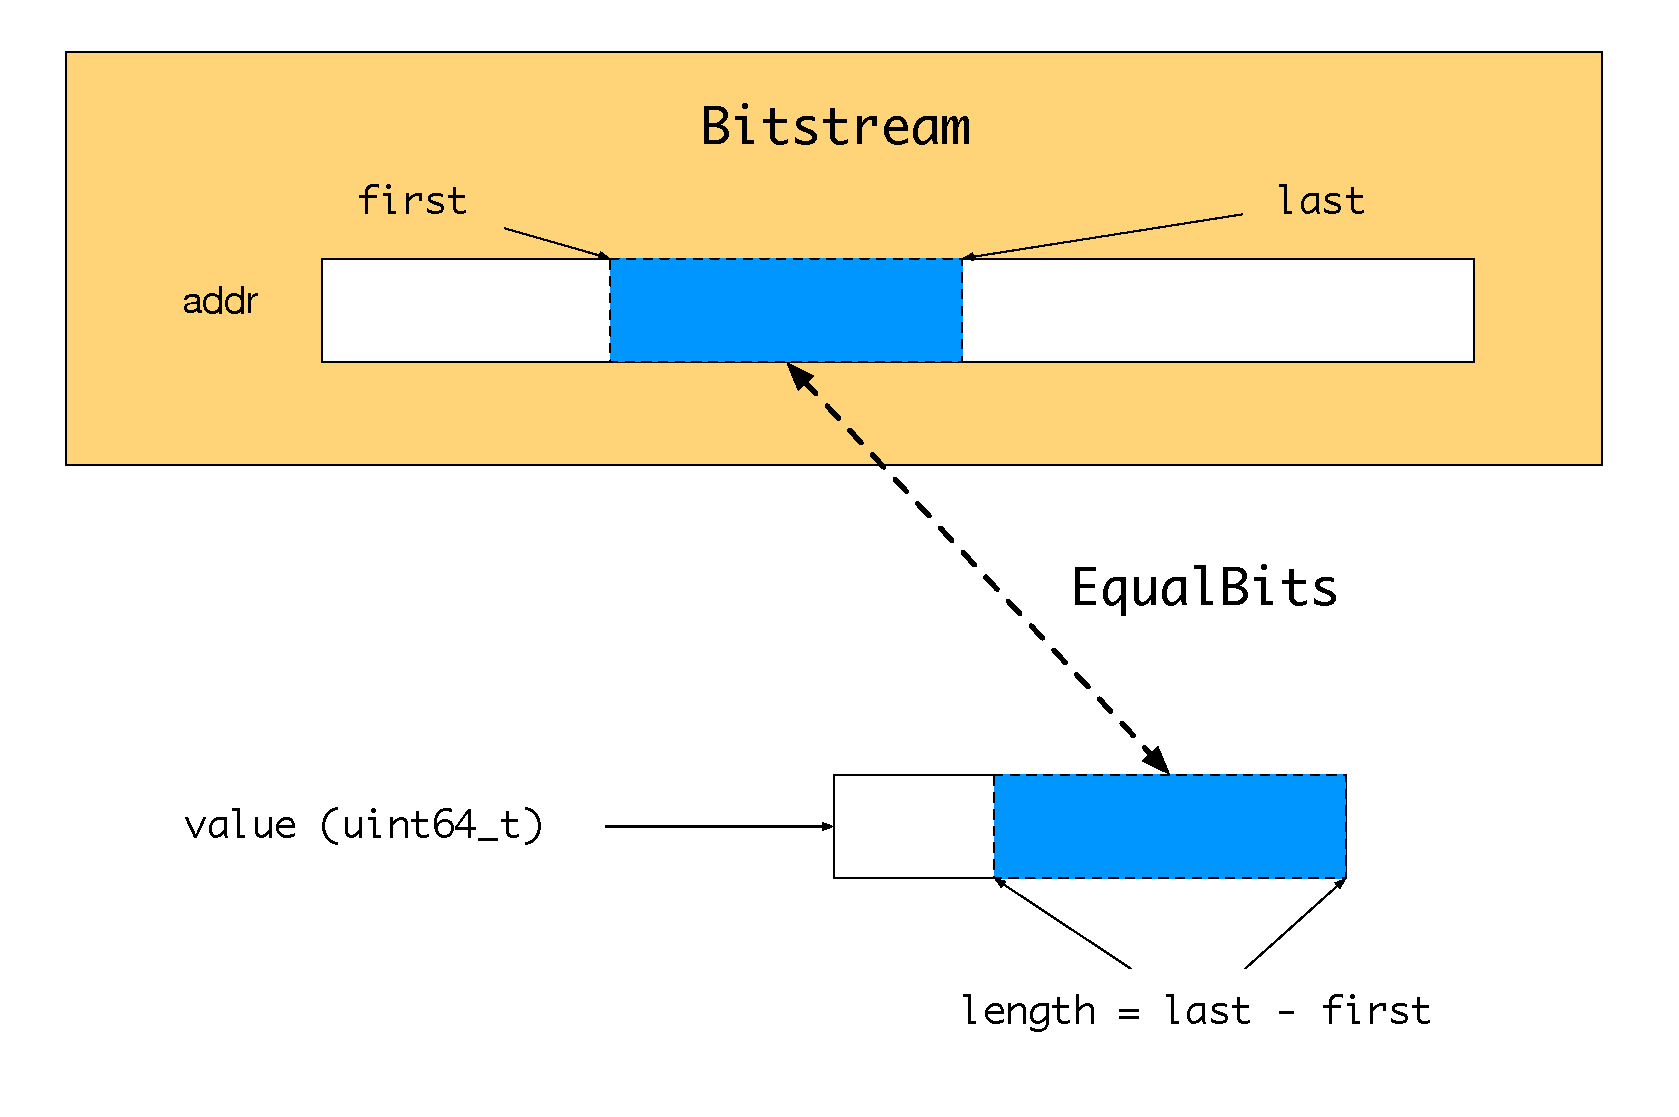
\includegraphics[width=0.99\textwidth]{figures/equalbits.pdf}
\caption{\label{fig:EqualBits correspondance}
	Bit coincidences required by \inl{EqualBits}}
\end{center}
\end{figure}



\section{Auxiliary \inl{Bitstream} functions}
\label{sec:bitstream-aux}


As a kind of constructor for type
\inl{Bitstream}, we provide the operation \inl{Bitstream_Init},
shown with its contract in Listing~\ref{lst:Bitstream_Init}.




\begin{listing}[hbt]
\begin{minipage}{0.99\textwidth}
\begin{lstlisting}[style=acsl-block]
/*@
  requires valid:     Writeable(stream);
  requires bit_size:  8 * size <= UINT32_MAX;
  requires valid_pos: bitpos <= 8 * size;
  requires separated: \separated(addr + (0..size-1), stream);

  assigns  stream->addr, stream->size, stream->bitpos;

  ensures  addr:      stream->addr == addr;
  ensures  size:      stream->size == size;
  ensures  bitpos:    stream->bitpos == bitpos;
  ensures  invariant: Invariant(stream, 0);
*/
void Bitstream_Init(Bitstream* stream, uint8_t* addr, uint32_t size, uint32_t bitpos);
\end{lstlisting}
\end{minipage}
\caption{\label{lst:Bitstream_Init}Setting-up a bitstream}
\end{listing}

\FloatBarrier

Moreover, we provide a test for exhaustion of a \inl{Bitstream},
shown in Listing~\ref{lst:Bitstream_Normal}.


\begin{listing}[hbt]
\begin{minipage}{0.99\textwidth}
\begin{lstlisting}[style=acsl-block]
/*@
  requires valid:     Readable(stream);
  requires invariant: Invariant(stream, length);

  assigns \nothing;

  ensures  result:    \result <==> Normal(stream, length);
*/
int Bitstream_Normal(const Bitstream* stream, uint32_t length);
\end{lstlisting}
\end{minipage}
\caption{\label{lst:Bitstream_Normal}Testing a bitstream for exhaustion}
\end{listing}



\FloatBarrier


\section{Writing bit sequences}
\label{sec:writing bit sequences}

In this section, we describe the operations that handle plain bit sequences.
%
They are used to implement the \inl{Bitstream} operations for
Section~\ref{sec:bitstream}.

Listing~\ref{lst:Bitstream_Write impl} shows contract of
the \inl{Bitstream_Write} operation,
and moreover exemplifies its implementation.


\begin{listing}[hbt]
\begin{minipage}{0.99\textwidth}
\begin{lstlisting}[style=acsl-block]
/*@
  requires valid:      Writeable(stream);
  requires invariant:  Invariant(stream, length);
  requires normal:     Normal(stream, length);
  requires upper:      UpperBitsNotSet(value, length);

  assigns stream->addr[0..stream->size - 1];
  assigns stream->bitpos;

  ensures  pos:        stream->bitpos == \old(stream->bitpos) + length;
  ensures  changed:    EqualBits(stream, \old(stream->bitpos), stream->bitpos, value);
  ensures  unchanged:  Unchanged{Here,Old}(stream, 0, \old(stream->bitpos));
  ensures  unchanged:  Unchanged{Here,Old}(stream, stream->bitpos, 8 * stream->size);
  ensures  size:       stream->size == \old(stream->size);
*/
void Bitstream_Write(Bitstream* stream, uint32_t length, uint64_t value)
{
    Bitwalker_Write(stream->addr, stream->size, stream->bitpos, length, value);
    //@ assert EqualBits(stream, stream->bitpos, stream->bitpos + length, value);

    stream->bitpos += length;
    //@ assert EqualBits(stream, \at(stream->bitpos,Pre), stream->bitpos, value);
}

\end{lstlisting}
\end{minipage}
\caption{\label{lst:Bitstream_Write impl}Writing to a bitstream}
\end{listing}

\FloatBarrier

Most parts of the contract are quite similar to that of
\inl{Bitstream_Read} in
Listing~\ref{lst:Bitstream_Read spec}.
%
Differences are the following:
\begin{itemize}
\item We require that the \inl{value} to be written fits into
	the specified
	\inl{length}, i.e.\ its unused most significant bits
	are zero (requirement property
	``\inl{upper}'').
\item The operation is allowed to change the contents of the bitstream
	(first \inl{assigns} clause) in addition to the streams
	current bit
	position (second \inl{assigns} clause), but no other
	memory locations.
\item Since we couldn't specify in the \inl{assigns} clauses 
	which bits exactly are allowed to be modified, we give the
	details in two
	\inl{ensures} clauses named ``\inl{unchanged}'':
	All bits before the stream's \inl{bitpos} on operation
	entry, and after
	its \inl{bitpos} on exit, must remain unchanged.
\end{itemize}

The implementation just employs the lower-level operation
\inl{Bitwalker_Write} to
write the bits, and appropriately updates the \inl{stream}'s
\inl{bitpos}.
%
Two assertions were needed to help the provers establishing that
\inl{value}'s
bits are actually written to \inl{stream}'s data array by

\fxfatal{something is missing here!!}


The formal definitions of the used \acsl predicates are given in
Listing~\ref{lst:Bitsequence preds}.
%
Again, the tacit assumption that the array contains sensible data
up to its very last bit is used in predicate \inl{Normal}.



\begin{listing}[hbt]
\begin{minipage}{0.99\textwidth}
\begin{lstlisting}[style=acsl-block]
/*@
   predicate Readable{L}(uint8_t* addr, integer size) = \valid_read(addr + (0..size-1));

   predicate Writeable{L}(uint8_t* addr, integer size) = \valid(addr + (0..size-1));

   predicate Invariant{L}(integer size, integer bitpos, integer length) =
       8 * size <= UINT32_MAX         &&
       length <= 64                   &&
       bitpos + length <= UINT32_MAX;

    predicate Normal{L}(integer size, integer bitpos, integer length) =
       bitpos + length <= 8 * size;
*/
\end{lstlisting}
\end{minipage}
\caption{\label{lst:Bitsequence preds} \acsl predicates used in bit sequence layer contracts}
\end{listing}


\FloatBarrier


Listing~\ref{Bitwalker_Write spec} shows the contract, and the
implementation, of the
\inl{Bitwalker_Write} operation.

\begin{listing}[hbt]
\begin{minipage}{0.99\textwidth}
\begin{lstlisting}[style=acsl-block]
/*@
  requires valid:      Writeable(addr, size);
  requires invariant:  Invariant(size, bitpos, length);
  requires normal:     Normal(size, bitpos, length);
  requires upper:      UpperBitsNotSet(value, length);

  assigns addr[0..size-1];

  ensures  left:       Unchanged{Here,Old}(addr, 0, bitpos);
  ensures  middle:     EqualBits(addr, bitpos, bitpos + length, value);
  ensures  right:      Unchanged{Here,Old}(addr, bitpos + length, 8 * size);
*/
void Bitwalker_Write(uint8_t* addr, uint32_t size, uint32_t bitpos, uint32_t length, uint64_t value);
{
    /*@
      loop invariant bound:   bitpos <= i <= bitpos + length;
      loop invariant left:    Unchanged{Here,Pre}(addr, 0, bitpos);
      loop invariant middle:  EqualBits(addr, bitpos, i, value, length);
      loop invariant right:   Unchanged{Here,Pre}(addr, i, 8 * size);

      loop assigns  i, addr[0..size-1];
      loop variant  bitpos + length - i;
    */
    for (uint32_t i = bitpos; i < bitpos + length; ++i)
    {
        int flag = TestBit64(value, (64 - length) + (i - bitpos));
        SetBit8Array(addr, size, i, flag);
    }   
}

\end{lstlisting}
\end{minipage}
\caption{\label{Bitwalker_Write spec}Writing a bit sequence}
\end{listing}

\FloatBarrier

\section{Reading bit sequences}
\label{sec:reading bit sequences}

The following peculiarities are observed when the former is
compared to \inl{Bitwalker_Read}'s contract in Listing~\ref{lst:Bitwalker_Read spec}.

\begin{listing}[hbt]
\begin{minipage}{0.99\textwidth}
\begin{lstlisting}[style=acsl-block]
/*@
  requires  valid:      Readable(addr, size);
  requires  invariant:  Invariant(size, bitpos, length);
  requires  normal:     Normal(size, bitpos, length);

  assigns   \nothing;

  ensures   equal:      EqualBits(addr, bitpos, bitpos + length, \result);
  ensures   upper:      UpperBitsNotSet(\result, length);
*/
uint64_t Bitwalker_Read(uint8_t* addr, uint32_t size, uint32_t bitpos, uint32_t length);
\end{lstlisting}
\end{minipage}
\caption{\label{lst:Bitwalker_Read spec}Reading a bit sequence}
\end{listing}

\FloatBarrier

\begin{itemize}
\item We require that the \inl{value} to be written fits into
the specific
	\inl{length}, i.e.\ all but its \inl{length}
	least significant bits are
	zero (requirement property ``\inl{upper}'').
\item The operation may modify the data array at \inl{addr},
but nothing else.
\item Again, we give the details of which data bits exactly
	are allowed to be changed in two
	\inl{ensures} clauses, named ``\inl{left}'' and
	``\inl{right}'', and requiring all bits before
	\inl{bitpos} and after
	\inl{bitpos+length} to remain unchanged, respectively.
\end{itemize}

In the implementation, which is shown here as an example, we used
the straight-forward
algorithm that takes a bit from \inl{value} and places it into
the \inl{addr} array, bit by bit.
%
In order for the provers to establish that algorithm's correctness,
we had to provide a total of six \acsl clauses about the loop:
%
\begin{itemize}
\item The loop variable, \inl{i}, always ranges in the interval
	[\inl{bitpos}\ldots\inl{bitpos+length}]---loop invariant property ``\inl{bound}''.
	%
	Note that the highest value is actually taken,
	viz.\ on exit of the loop body in the last iteration,
	subsequently causing the loop to terminate.
\item The bits before \inl{bitpos}, and after
	\inl{bitpos+length}
	remain as they were on operation entry---invariant property
	``\inl{left}'' and ``\inl{right}'', respectively.
\item In the \inl{i}th iteration, the bits
	[\inl{bitpos}\ldots\inl{bitpos+i}) agree with
	the least significant
	\inl{i} bits of \inl{value}---invariant property
	``\inl{middle}''.
\item The loop code is allowed to modify the variable \inl{i},
	and the whole array
	at \inl{addr}, but nothing else---
	\inl{loop assigns} clause.
\item The value of the integer
	expression \inl{bitpos+length-i} is non-negative throughout
	the whole loop execution, but is decreased in every iteration 
	--- \inl{loop variant} clause.
	%
	Therefore, the loop is guaranteed to terminate eventually.
\end{itemize}




The operations we have discussed here are based
on operations to write and to read a single bit.
%
The details of the latter, as well as of the predicates used in their
contracts, are given in Appendix~\ref{cha:low-level bitstream}.


\section{Verification of the Bitstream abstraction}
\label{sec:bitstream verif}



Critics of the formal software verification approach often 
argue that verifying an operation against its formal specification
results in little or no increase of trustworthiness when
%
\begin{itemize}
\item the specification, including all auxiliary definitions etc., is
	as complex as the operation's implementation, or/and
\item the specification essentially duplicates the implemented
	algorithm in a different (such as functional rather than
	imperative) language.
\end{itemize}
%
Both criteria may be seen to be met by our Bitwalker case study.



However, since the operations we dealt with essentially implement a
communication protocol, there is a very simple ``high-level'' property
that should be satisfied, viz.\ that a ``send'' operation is inverse
to a ``receive'' operation.
%
This property can be stated formally in a very brief and understandable
way.
%
It ensures, in a mathematical context, that both operations implement
bijective mappings, that is, in an engineering sense, that the
communication channel neither looses, nor subjoins information.
%
In fact, we have achieved to formally prove this property.




More particularly, in our setting, we could show that the operations
\inl{Bitstream_Read} and \inl{Bitstream_Write} are
inverse to each other.
%
To this end, we set up two fictitious \isoc procedures realizing
the composition of both operations in the two possible orders.




Listing~\ref{lst:Bitstream_WriteThenRead}
shows the procedure for the scenario ``use \inl{Bitstream_Write}
to write a value to a stream, then immediately read it back using
\inl{Bitstream_Read}''.


\begin{listing}[hbt]
\begin{minipage}{0.99\textwidth}
\begin{lstlisting}[style=acsl-block]
/*@
    requires valid:      Writeable(stream);
    requires invariant:  Invariant(stream, length);
    requires normal:     Normal(stream, length);
    requires upper:      UpperBitsNotSet(value, length);

    assigns stream->addr[0..stream->size-1];
    assigns stream->bitpos;

    ensures equality:     \result == value;
*/
uint64_t Bitstream_WriteThenRead(Bitstream* stream, uint32_t length, uint64_t v>
{
    //@ ghost uint32_t old_pos = stream->bitpos;

    Bitstream_Write(stream, length, value);
    //@ assert equal:  EqualBits(stream, old_pos, old_pos+length, value);

    /*@ 
        assigns stream->bitpos;
        ensures reset: stream->bitpos == \at(stream->bitpos,Pre);
    */
    stream->bitpos -= length;

    uint64_t result = Bitstream_Read(stream, length);
    //@ ghost uint32_t new_pos = stream->bitpos;
    //@ assert equal_result: EqualBits(stream, old_pos, new_pos, result);
    //@ assert equal_value:  EqualBits(stream, old_pos, new_pos, value);
    /*@ assert aux:          \forall integer k; old_pos <= k < new_pos ==>
                               \let j = new_pos - 1 - k;
                               (BitTest(value,  j) <==> BitTest(result, j));
    */
    //@ assert left:         EqualBits64(result, value, 64-length, 64);
    //@ assert compare:      EqualBits64(result, value, 0, 64);

    return result;
}
\end{lstlisting}
\end{minipage}
\caption{\label{lst:Bitstream_WriteThenRead}
	Verifying the scenario ``write, then read'' }
\end{listing}

\FloatBarrier

The procedure's body code is straightforward; after
\inl{Bitstream_Write}, we have to seek back to the original bit
position, before calling \inl{Bitstream_Read}''.
%
We could show that the read value always equals the written one,
provided
\begin{itemize}
\item the stream is accessible for both read and update
	(requirement property ``\inl{valid}''),
\item it satisfies its type invariant (property
	``\inl{invariant}''; cf.\ Listing~\ref{lst:Bitstream preds}
	and~\ref{lst:Bitsequence preds}),
\item the stream's current bit position is sufficiently small such that
	all value bits still fit into the stream
	(property``\inl{normal}''), and
\item the most significant value bits that are not written are all zero
	(property``\inl{upper}'').
\end{itemize}
%
This ensures that the bitstream communication channel doesn't loose
information---every value we write into it can completely be
restored.



Vice versa, we could also show that the channel doesn't transmit more
information than is needed to fulfill its task.
%
Listing~\ref{lst:Bitstream_ReadThenWrite}
shows the procedure for the scenario ``use \inl{Bitstream_Read}
to read a value from a stream, then immediately write it back using
\inl{Bitstream_Write}''.




\begin{listing}[hbt]
\begin{minipage}{0.99\textwidth}
\begin{lstlisting}[style=acsl-block]
/*@
    requires valid:      Writeable(stream);
    requires invariant:  Invariant(stream, length);
    requires normal:     Normal(stream, length);

    assigns stream->addr[0..stream->size-1];
    assigns stream->bitpos;

    ensures  unchanged:  Unchanged{Here,Old}(stream, 0, 8 * stream->size);
*/
void Bitstream_ReadThenWrite(Bitstream* stream, uint32_t length)
{
    //@ ghost uint32_t old_pos = stream->bitpos;
    uint64_t value = Bitstream_Read(stream, length);
    //@ assert equal:  EqualBits(stream, old_pos, old_pos+length, value);

    stream->bitpos -= length;
    //@ assert stream->bitpos == old_pos;

    Bitstream_Write(stream, length, value);
    //@ assert unchanged:  Unchanged{Here,Pre}(stream, old_pos, stream->bitpos);
}
\end{lstlisting}
\end{minipage}
\caption{\label{lst:Bitstream_ReadThenWrite}
	Verifying the scenario ``read, then write'' }
\end{listing}


\FloatBarrier


We were able show that this leaves the
whole stream unchanged, provided the first three requirement properties
from \inl{Bitstream_WriteThenRead} are met.
%
As an example for a channel transmitting redundant information,
consider
a bitstream implementation
with \inl{Bitstream_Write}
storing each byte twice in succession and \inl{Bitstream_Read}
ignoring every second byte.
%
Such a stream doesn't meet our property, since, 
starting from a stream with non-agreeing adjacent bytes, there is no
way to reproduce it by a ``read, then write'' scenario.
\cleardoublepage

\chapter{Low-level bitstream operations}
\label{cha:low-level bitstream}

In this appendix, we describe the implementation of the
low-level bitstream operations.
%
They were used to implement the bit sequence abstraction level, cf.\
Chapter~\ref{cha:bitstream}.
%
Since a write operation moves bits from a \inl{uint64_t} value
into an array of \inl{uint8_t} values, and a read operations
moved them the other way round,
we need bit operations on both data types.
%
They are given in
Subsection~\ref{subsec:low-level 8 array} 
for an array of \inl{uint8_t}, 
in Subsection~\ref{subsec:low-level 8} for a single \inl{uint8_t},
and
in Subsection~\ref{subsec:low-level 64} for single \inl{uint64_t}.













\section{Reading and writing individual bits}


\subsection{8 bit arrays}
\label{subsec:low-level 8 array}


In this section, we discuss the operations for read and write of a
single bit from/into a byte array.

The operation \inl{TestBit8Array(addr,size,pos)} returns the
\inl{pos}$^{\mbox{\scriptsize th}}$ bit
within the array at \inl{addr}
of byte-size \inl{size}.\footnote{
	This parameter isn't actually used in the code, but merely
	in the contract.
}
Its contract and its implementation is shown in
Listing~\ref{lst:TestBit8Array}.
%
See Listing~\ref{lst:bit predicate defs} for the definition of the predicate
\inl{Bit8Array}.
%
The array bits are counted starting with the most significant one of
the first byte,
cf.\ Figure~\ref{fig:bit coords} below.
%
A call to \inl{TestBit8(bytevalue,bitadr)} returns the 
\inl{bitadr}$^{\mbox{\scriptsize th}}$ bit
within \inl{bytevalue}, this operation is discussed in
Appendix~\ref{subsec:low-level 8} below.








\begin{listing}[hbt]
\begin{minipage}{0.99\textwidth}
\begin{lstlisting}[style=acsl-block]
/*@
    requires valid:  \valid_read(addr + (0..size-1));
    requires size:   8 * size <= UINT32_MAX;
    requires pos:    pos < 8 * size;

    assigns \nothing;

    ensures result:  \result != 0 <==> Bit8Array(addr, pos);
*/
static inline int TestBit8Array(uint8_t*  addr, uint32_t size, uint32_t pos)
{
    return TestBit8(addr[pos / 8], pos % 8);
}
\end{lstlisting}
\end{minipage}
\caption{\label{lst:TestBit8Array}Reading a bit of an \inl{uint8_t} array}
\end{listing}










Similarly, the operation \inl{SetBit8Array(addr,size,pos,flag)}
sets the
\inl{pos}$^{\mbox{\scriptsize th}}$ bit within the array at
\inl{addr} of
byte-size \inl{size} to \inl{flag}.
%
Its contract is shown in Listing~\ref{lst:SetBit8Array}.
%
It requires
%
\begin{itemize}
\item the whole array to be accessible for update (requirement
	property ``\inl{valid}''),
\item each possible bit position in the array to fit into a
	\inl{uint32_t} (property ``\inl{size}''), and
\item the given \inl{pos} to be a valid bit position in the array
	(property ``\inl{pos}'').
\end{itemize}
%
The \inl{assigns} clause allows the operation to change the
contents of the array,
but no other memory locations.
%
On completion, the operation shall guarantee
\begin{itemize}
\item that the value of \inl{flag}\footnote{
		Any non-zero \inl{flag} value is treated like 1.
		This is ensured by the contract of the called operation
		\inl{SetBit8}, cf.\ Appendix~\ref{subsec:low-level 8}.
	}
	is actually stored at the designated bit
	position (postcondition property ``\inl{middle}'';
	the call \inl{Bit8Array()} succeeds if, and inly if, the
	\inl{pos}$^{\mbox{\scriptsize th}}$ bit within the byte
	array at \inl{addr} is set, 
	cf.\ Listing~\ref{lst:bit predicate defs} in
	Appendix~\ref{sec:bit operations in framac}), and
\item that all other bits remain unchanged 
	(properties ``\inl{left}'', ``\inl{right}'').
\end{itemize}
%
Two fairly sophisicated hints had to be provided as assertions in
the body in order for
the provers to establish the contract's post-conditions.









\begin{listing}[hbt]
\begin{minipage}{0.99\textwidth}
\begin{lstlisting}[style=acsl-block]
/*@
    requires valid:  \valid(addr + (0..size-1));
    requires size:   8 * size <= UINT32_MAX;
    requires pos:    pos < 8 * size;

    assigns addr[0..size-1];

    ensures left:   Unchanged{Here,Old}(addr, 0, pos);
    ensures middle: Bit8Array(addr, pos) <==> (flag != 0);
    ensures right:  Unchanged{Here,Old}(addr, pos + 1, 8 * size);
*/
static inline void SetBit8Array(uint8_t* addr, uint32_t size, uint32_t pos, int flag)
{
    uint32_t i = pos / 8u;
    uint32_t k = pos % 8u;

    addr[i] = SetBit8(addr[i], k, flag);

    // The following assertion claims that in byte with index "pos/8"
    // the bits with indices different from "k" do not change
    /*@
      assert bits_in_byte:
        \forall integer j; (0 <= j < 8  && j != k) ==>
        (Bit8(addr[pos/8], j) <==> \at(Bit8(addr[pos/8], j), Pre));
    */

    // The following assertion claims that in every byte
    // with an index that is different from "pos/8" no bit is changed.

    /*@
        assert other_bytes:
        \forall integer l, j; (0 <= l < size  &&  l != pos/8  &&  0 <= j < 8) ==>
          (Bit8(addr[l], j) <==> \at(Bit8(addr[l], j), Pre));
    */

}
\end{lstlisting}
\end{minipage}
\caption{\label{lst:SetBit8Array}Writing a bit of an \inl{uint8_t} array}
\end{listing}








\FloatBarrier

\subsection{8 bits}
\label{subsec:low-level 8}









\begin{listing}[hbt]
\begin{minipage}{0.99\textwidth}
\begin{lstlisting}[style=acsl-block]
/*@
    requires pre:  pos < 8;

    assigns \nothing;

    ensures pos:  \result != 0 <==> Bit8(value, pos);
*/
static inline int TestBit8(uint8_t value, uint32_t pos)
{
    uint8_t mask = ((uint8_t) 1) << (7u - pos);
    uint8_t flag = value & mask;

    return flag != 0;
}
\end{lstlisting}
\end{minipage}
\caption{\label{lst:TestBit8}Reading a bit of \inl{uint8_t}}
\end{listing}










The operation \inl{TestBit8(value,pos)} returns the
\inl{pos}$^{\mbox{\scriptsize th}}$
bit of \inl{value}.
%
Its contract is shown in Listing~\ref{lst:TestBit8}.
%
\begin{itemize}
\item The value of \inl{pos} must not exceed 7 
	(requirement property ''\inl{pre}''),
\item no memory may be modified (\inl{assigns}), and 
\item the result is non-zero if, and only
	if, the specified bit is set (postcondition property
	``\inl{pos}''; the call \inl{Bit8(value,pos)} succeeds 
	if, and only if, the \inl{pos}$^{\mbox{\scriptsize th}}$ of
	the byte \inl{value} is set, 
	cf.\ Listing~\ref{lst:bit predicate defs} in
	Appendix~\ref{sec:bit operations in framac}).
\end{itemize}
%
The shown implementation additionally guarantees that the result is
zero or one, which
is not specified in the contract since this property isn't needed.
%
Returning just \inl{flag} rather than \inl{flag!=0u}
would satisfy the
contract also, and would be slightly faster.






Dual to \inl{TestBit8}, the operation
\inl{SetBit8(value,pos,flag)}
returns \inl{value}, 
with the \inl{pos}$^{\mbox{\scriptsize th}}$ bit
set to \inl{flag}.
%
Its contract is shown in Listing~\ref{lst:SetBit8}.
%
\begin{itemize}
\item Again, the value of \inl{pos} mustn't exceed 7 
	(requirement property ``\inl{pre}''),
\item no memory may be modified (\inl{assigns} clause),
\item the return value coincides with \inl{value}, except possibly
	at \inl{pos} (postcondition properties ``\inl{left}'' 
	and ``\inl{right}''; a call
	\inl{EqualBits8(x,y,first,last)} succeeds if, and
	only if, the \inl{uint8_t} values \inl{x} and
	\inl{y} agree on all bits in range
	[\inl{first}\ldots\inl{last}), cf.\ also
	Listing~\ref{lst:EqualBits64} in 
	Appendix~\ref{sec:bit operations in framac}), and 
\item \inl{flag} is written to the approriate bit of 
	\inl{value} (property ``\inl{pos}'').
\end{itemize}
%
The implementation branches on the value of \inl{flag}, and
clears or sets the
appropriate bit in the usual way.
%
Note that both our contract and our implementation enable us to set
a bit by supplying a
\inl{flag} value of e.g.\ 2, whereas the code 
``\inl{mask=flag<<(7-pos);return(value&~mask)|mask}'' does not.





\begin{listing}[hbt]
\begin{minipage}{0.99\textwidth}
\begin{lstlisting}[style=acsl-block]
/*@
    requires pre: pos < 8;

    assigns \nothing;

    ensures left:   EqualBits8(\result, value, 0,  pos);
    ensures pos:    Bit8(\result, pos) <==> (flag != 0);
    ensures right:  EqualBits8(\result, value, pos + 1,  8);
*/
static inline uint8_t SetBit8(uint8_t value, uint32_t pos, int flag)
{
    uint8_t mask = ((uint8_t) 1) << (7u - pos);

    return (flag == 0) ? (value & ~mask) : (value | mask);
}
\end{lstlisting}
\end{minipage}
\caption{\label{lst:SetBit8}Writing a bit of \inl{uint8_t}}
\end{listing}





















\FloatBarrier

\subsection{64 bits}
\label{subsec:low-level 64}



The operations to read and write a bit of a \inl{uint64_t}
are closely similar to
those working on a \inl{uint8_t}.
%
They are shown in Listing~\ref{lst:TestBit64}
and \ref{lst:SetBit64} without repeating the comments given
in Appendix~\ref{subsec:low-level 8} for the 8 bit version.
%
See Listing~\ref{lst:bit predicate defs} for the employed ACSL predicates.





\begin{listing}[hbt]
\begin{minipage}{0.99\textwidth}
\begin{lstlisting}[style=acsl-block]
/*@
   requires pre: pos < 64;

   assigns \nothing;

   ensures set_bit: \result != 0 <==> Bit64(value, pos);
*/
int TestBit64(uint64_t value, uint32_t pos)
{
    uint64_t mask = ((uint64_t) 1) << (63u - pos);
    uint64_t flag = value & mask;

    return flag != 0u;
}
\end{lstlisting}
\end{minipage}
\caption{\label{lst:TestBit64}Reading a bit of \inl{uint64_t}}
\end{listing}








Listing~\ref{lst:SetBit64} shows the operation \inl{SetBit64}.
%
Note that it has a redundant postcondition, viz.\ property
``\inl{upper}'', which guarantees that the leading zeros in
\inl{value} are kept in the result, up to, but excluding
position \inl{pos}.
%
This property was needed to enable the provers to verify code that uses
\inl{SetBit64}.




\begin{listing}[hbt]
\begin{minipage}{0.99\textwidth}
\begin{lstlisting}[style=acsl-block]
/*@
    requires pre: pos < 64;

    assigns \nothing;

    ensures left:     EqualBits64(\result, value, 0,  pos);
    ensures set_bit:  flag != 0  <==>  Bit64(\result, pos);
    ensures right:    EqualBits64(\result, value, pos + 1,  64);
    ensures upper:    \forall integer i; i >= 64 - pos ==>
                         (UpperBitsNotSet(value, i) ==> UpperBitsNotSet(\result, i));
*/
uint64_t SetBit64(uint64_t value, uint32_t pos, int flag)
{
    uint64_t mask = ((uint64_t) 1u) << (63 - pos);

    return (flag == 0) ? (value & ~mask) : (value | mask);
}
\end{lstlisting}
\end{minipage}
\caption{\label{lst:SetBit64}Writing a bit of \inl{uint64_t}}
\end{listing}




The operation \inl{UpperBitsNotSet64(value,length)} succeeds,
i.e.\ returns a
non-zero value, if, and only if, all bits of \inl{value} except
the least significant
\inl{length} ones are zero.
%
It is used in the implementation of packet writing functions like
\inl{AdhesionFactor_EncodeBit} 
%\fxfatal{oder doch AdhesionFactor\_EncodeBit ?}
(see Section~\ref{sec:adhesionfactor-encodebit})
to check that no non-zero bits from the packet structure (like
\inl{struct AdhesionFactor}) are ignored due to space
limitations in the bitstream.





\begin{listing}[hbt]
\begin{minipage}{0.99\textwidth}
\begin{lstlisting}[style=acsl-block]
/*@
    requires pre: length <= 64;

    assigns \nothing;

    ensures  not_set: \result <==> UpperBitsNotSet(value, length);
*/
int UpperBitsNotSet64(uint64_t value, uint32_t length);
\end{lstlisting}
\end{minipage}
\caption{\label{lst:UpperBitsNotSet64}Test that upper bits are not set}
\end{listing}
% BODY OMITTED:
%{
%    if (length == 64)
%    {
%        return 1;
%    }
%    else
%    {
%        const uint64_t MaxValue = ((uint64_t) 1) << length;
%        // assert equiv: UpperBitsNotSet(value, length) <==> value < MaxValue;
%
%        return value < MaxValue;
%    }
%}











\FloatBarrier

\section{Formalization of bit operations in \framac}
\label{sec:bit operations in framac}






The definition of predicate \inl{Bit8} is shown in 
Listing~\ref{lst:bit predicate defs}.
%
It relies on the Frama-C library predicate \inl{BitTest},
performing a coordinate
transformation to fit Frama-C's notion of bit positions with the
OpenETCS project's
notion, cf.\ Figure~\ref{fig:bit coords}.





\begin{listing}[hbt]
\begin{minipage}{0.99\textwidth}
\begin{lstlisting}[style=acsl-block]
/*@
   predicate Bit8{A}(uint8_t v, integer n)  = BitTest(v, 7 - n);

   predicate Bit64{A}(uint64_t v, integer n) = BitTest(v, 63 - n);

   predicate Bit8Array{A}(uint8_t* a, integer n) = Bit8(a[n / 8],n % 8);
*/
\end{lstlisting}
\end{minipage}
\caption{\label{lst:bit predicate defs}Definition of bit test predicates}
\end{listing}













\begin{figure}
\begin{center}
\vspace*{2cm}
--- Insert drawing --- 
\vspace*{2cm}
\caption{\label{fig:bit coords}
        Bit coordinates in Frama-C and in the OpenETCS project}
\end{center}
\end{figure}






The predicate \inl{UpperBitsNotSet(value,length)} succeeds if,
and only if,
all but possibly 
the least significant \inl{length} bits of \inl{value} are zero.
%
Its definition is shown in Listing~\ref{lst:UpperBitsNotSet integer}.







\begin{listing}[hbt]
\begin{minipage}{0.99\textwidth}
\begin{lstlisting}[style=acsl-block]
predicate
  UpperBitsNotSet{A}(integer value, integer length) =
    \forall integer i; length <= i ==> !BitTest(value, i);
\end{lstlisting}
\end{minipage}
\caption{\label{lst:UpperBitsNotSet integer}
	Definition of the low-level predicate \inl{UpperBitsNotSet}}
\end{listing}


Listing~\ref{lst:EqualBits64} shows the predicate
\inl{EqualBits64} that was used in the 64-bit
operations' contracts.
%
The call \inl{EqualBits64(x,y,first,last)} succeeds if, and inly
if, the \inl{uint64_t} values  \inl{x} and  \inl{y}
agree on all bits in the range from \inl{first} to \inl{last}).
%
The predicate \inl{EqualBits8}, used in
Appendix~\ref{subsec:low-level 8}, is defined in similar way; its
definition need not be shown here.










\begin{listing}[hbt]
\begin{minipage}{0.99\textwidth}
\begin{lstlisting}[style=acsl-block]
/*@
   predicate
     EqualBits64{A}(uint64_t x, uint64_t y, integer first, integer last) =
        \forall integer i; 64 - last <= i < 64 - first 
          ==> (BitTest(x, i) <==> BitTest(y, i));
\end{lstlisting}
\end{minipage}
\caption{\label{lst:EqualBits64}
        Definition of the low-level predicate \inl{EqualBits64}}
\end{listing}








In order for the provers to find all low-level validation proofs, we
needed to supply three redundand properties about
\inl{EqualBits64} and \inl{UpperBitsNotSet}; they are shown
in Listing~\ref{lst:axioms64}.
%
Axiom \inl{equal_bits64_0} states that two \inl{uint64_t}
values must be equal, if they agree on all 64 bit positions.
%
Axiom \inl{upper_bits_less_than} states that in a nonnegative number
less than $2^n$ all bits are zero, except for possibly
the least significant \inl{n} ones.
%
The neccessity of these extra axioms might indicate an
incompleteness in Frama-C's actual bit-operator theory; this is currently
investigated.
%
Axiom \inl{equal_bits64_1} is just a (relaxed)
rephrasing of the definition
in Listing~\ref{lst:EqualBits64}, using a different index scheme.
%
It is necessary due to the provers' weakness in applying index
transformations.










\begin{listing}[hbt]
\begin{minipage}{0.99\textwidth}
\begin{lstlisting}[style=acsl-block]
   axiomatic BitProperties
   {
     axiom equal_bits64_0:
       \forall uint64_t x, y;
         EqualBits64(x, y, 0, 64) ==> x == y;

     axiom equal_bits64_1:
       \forall uint64_t x, y, integer p, q;
         (\forall integer k; p <= k < q 
           ==> \let j = q-1-k; (BitTest(x, j) <==> BitTest(y, j)))
         ==> EqualBits64(x, y, 64-(q-p), 64);

      axiom upper_bits_less_than:
        \forall integer x, n; x >= 0 ==> n >= 0 ==>
           (UpperBitsNotSet(x, n) <==> x < (1 << n));
   }
*/
\end{lstlisting}
\end{minipage}
\caption{\label{lst:axioms64}ACSL axioms used in 64-bit contracts}
\end{listing}








For a nonnegative integer \inl{v},
the predicate \inl{BitTest(v,n)} succeeds if, and only if, the
\inl{n}$^{\mbox{\scriptsize th}}$ bit is set in the binary
representation of
\inl{v}, i.e.\ iff the truncating integer division of \inl{v} by
$2^{\mbox{\scriptsize\inl{n}}}$ yields an odd number.
%
This predicate comes with the standard library of the Frama-C system,
however, without any detailled documentation.
%
Its declaration is shown in Listing~\ref{lst:BitTest}.


\begin{listing}[hbt]
\begin{minipage}{0.99\textwidth}
\begin{lstlisting}[style=acsl-block]
/*@
   predicate   BitTest(integer v, integer n);
*/
\end{lstlisting}
\end{minipage}
\caption{\label{lst:BitTest}
	The Frama-C library predicate \inl{BitTest}}
\end{listing}











%	\begin{listing}[hbt]
%	\begin{minipage}{0.99\textwidth}
%	\begin{lstlisting}[style=acsl-block]
%	
%	\end{lstlisting}
%	\end{minipage}
%	\caption{caption}
%	\end{listing}

\cleardoublepage

\chapter{Formal verification}
\label{cha:formal-verification}

\section{Bit stream and lower-level bit operations}
\label{sec:bitstream-verification}

\begin{table}[hbt]
\begin{center}
    \begin{tabular}{|l|ccc|cccc|}
\hline
\multirow{2}{*}{\textbf{component}} &
\multicolumn{3}{c|}{ \textbf{vcs}} &
\multicolumn{4}{c|}{\textbf{individual provers}}\\
\cline{2-8}
               &  all & proven & (\%) & qed & alt-ergo & cvc4 & z3  \\
\hline
\hline
bit stream     & 58 &  58 & 100 & 19 &  0 & 0 & 39  \\
\hline
bit stream (inverse)  & 58 & 58 & 100 & 33 &  2 & 1 & 22  \\
\hline
lower-level bit ops & 126 & 126 & 100 & 55 &  0 & 1 & 70  \\
\hline
\end{tabular}
\end{center}
\caption{\label{tbl:bitstream-verification} verfication result for bit stream and lower-level bit operations}
\end{table}

\FloatBarrier  % forces the output of listings/tables

\section{Verification of packets without \inl{N_ITER}}
\label{sec:packets-without-niter-verification}


\begin{table}[hbt]
\begin{center}
    \begin{tabular}{|m{10ex}|m{5ex}m{5ex}m{5ex}|m{5ex}m{5ex}m{5ex}m{5ex}|}
\hline
\multirow{2}{*}{\textbf{PacketID}} &
\multicolumn{3}{c|}{ \textbf{VCs}} &
\multicolumn{4}{c|}{\textbf{Individual Provers}}\\
\cline{2-8}
               &  All & Proven & (\%) & Qed & Alt-Ergo & CVC4 & Z3  \\
\hline
\hline
16 & 436 & 436 & 100 & 318 & 0 & 1 & 117\\
\hline
39 & 483 & 483 & 100 & 346 & 0 & 1 & 136\\
\hline
42 & 559 & 543 & 97 & 399 & 0 & 1 & 143\\
\hline
45 & 389 & 389 & 100 & 290 & 0 & 1 & 98\\
\hline
57 & 483 & 483 & 100 & 346 & 0 & 1 & 136\\
\hline
65 & 624 & 624 & 100 & 430 & 0 & 1 & 193\\
\hline
66 & 389 & 389 & 100 & 290 & 0 & 1 & 98\\
\hline
71 & 530 & 530 & 100 & 374 & 0 & 1 & 155\\
\hline
72 & 999 & 957 & 95 & 671 & 0 & 1 & 285\\
\hline
76 & 958 & 938 & 97 & 644 & 9 & 1 & 284\\
\hline
90 & 474 & 465 & 98 & 341 & 0 & 1 & 123\\
\hline
\end{tabular}
\end{center}
\caption{\label{tbl:packets-without-niter-tracktotrain-part1} Verfication result for TrackToTrain packets without \inl{N_ITER} part 1}
\end{table}

\FloatBarrier  % forces the output of listings/tables

\begin{table}[hbt]
\begin{center}
    \begin{tabular}{|m{10ex}|m{5ex}m{5ex}m{5ex}|m{5ex}m{5ex}m{5ex}m{5ex}|}
\hline
\multirow{2}{*}{\textbf{PacketID}} &
\multicolumn{3}{c|}{ \textbf{VCs}} &
\multicolumn{4}{c|}{\textbf{Individual Provers}}\\
\cline{2-8}
               &  All & Proven & (\%) & Qed & Alt-Ergo & CVC4 & Z3  \\
\hline
\hline
131 & 624 & 624 & 100 & 430 & 0 & 1 & 193\\
\hline
132 & 389 & 389 & 100 & 290 & 0 & 1 & 98\\
\hline
133 & 718 & 718 & 100 & 486 & 0 & 1 & 231\\
\hline
134 & 624 & 624 & 100 & 430 & 0 & 1 & 193\\
\hline
136 & 474 & 465 & 98 & 341 & 0 & 1 & 123\\
\hline
137 & 389 & 389 & 100 & 290 & 0 & 1 & 98\\
\hline
138 & 483 & 483 & 100 & 346 & 0 & 1 & 136\\
\hline
139 & 483 & 483 & 100 & 346 & 0 & 1 & 136\\
\hline
140 & 389 & 389 & 100 & 290 &  0 &  1 & 98\\
\hline
141 & 436 & 436 & 100 & 318 & 0 & 1 & 117\\
\hline
254 & 342 & 342 & 100 &262 & 0 & 1 & 79\\
\hline
\end{tabular}
\end{center}
\caption{\label{tbl:packets-without-niter-tracktotrain-part2} Verfication result for TrackToTrain packets without \inl{N_ITER} part 2}
\end{table}

\FloatBarrier  % forces the output of listings/tables

\begin{table}[hbt]
\begin{center}
    \begin{tabular}{|m{10ex}|m{5ex}m{5ex}m{5ex}|m{5ex}m{5ex}m{5ex}m{5ex}|}
\hline
\multirow{2}{*}{\textbf{PacketID}} &
\multicolumn{3}{c|}{ \textbf{VCs}} &
\multicolumn{4}{c|}{\textbf{Individual Provers}}\\
\cline{2-8}
               &  All & Proven & (\%) & Qed & Alt-Ergo & CVC4 & Z3  \\
\hline
\hline
1 & 973 & 948 & 97 & 649 & 6 & 2 & 291\\
\hline
4 & 342 & 342 & 100 & 262 & 0 & 1 & 79\\
\hline
9 & 342 & 342 & 100 & 262 & 0 & 1 & 79\\
\hline
44 & 389 & 389 & 100 & 290 & 0 & 1 & 98\\
\hline
\end{tabular}
\end{center}
\caption{\label{tbl:packets-without-niter-traintotrack} Verfication result for TrainToTrack packets without \inl{N_ITER}}
\end{table}

\FloatBarrier  % forces the output of listings/tables

\begin{table}[hbt]
\begin{center}
    \begin{tabular}{|m{10ex}|m{5ex}m{5ex}m{5ex}|m{5ex}m{5ex}m{5ex}m{5ex}|}
\hline
\multirow{2}{*}{\textbf{PacketID}} &
\multicolumn{3}{c|}{ \textbf{VCs}} &
\multicolumn{4}{c|}{\textbf{Individual Provers}}\\
\cline{2-8}
               &  All & Proven & (\%) & Qed & Alt-Ergo & CVC4 & Z3  \\
\hline
\hline
255 & 239 & 239 & 100 & 192 & 0 & 1 & 46\\
\hline
\end{tabular}
\end{center}
\caption{\label{tbl:packets-without-niter-bothways} Verfication result for BothWays packets without \inl{N_ITER}}
\end{table}

\FloatBarrier  % forces the output of listings/tables

\begin{table}[hbt]
\begin{center}
    \begin{tabular}{|m{8ex}|m{11cm}|m{9ex}|m{11ex}|}
\hline
               PacketID & Packetname & \inl{N_ITER} & Conditionals\\
\hline
\hline
3 & \inl{NationalValues} & dynamic & conditional\\
\hline
5 & \inl{Linking} & dynamic & conditional\\
\hline
12 & \inl{Level1MovementAuthority} & dynamic & -\\
\hline
15 & \inl{Level23MovementAuthority} & dynamic & -\\
\hline
16 & \inl{RepositioningInformation} & static & -\\
\hline
21 & \inl{GradientProfile} & dynamic & -\\
\hline
27 & \inl{InternationalStaticSpeedProfile} & dynamic & -\\
\hline
39 & \inl{TrackConditionChangeOfTractionPower} & static & -\\
\hline
41 & \inl{LevelTransitionOrder} & dynamic & conditional\\
\hline
42 & \inl{SessionManagement} & static & conditional\\
\hline
45 & \inl{RadioNetworkRegistration} & static & -\\
\hline
46 & \inl{ConditionalLevelTransitionOrder} & dynamic & conditional\\
\hline
49 & \inl{ListOfBalisesForSHArea} & dynamic & conditional\\
\hline
51 & \inl{AxleLoadSpeedProfile} & dynamic & -\\
\hline
57 & \inl{MovementAuthorityRequestParameters} & static & -\\
\hline
58 & \inl{PositionReportParameters} & dynamic & -\\
\hline
63 & \inl{ListOfBalisesInSRAuthority} & dynamic & conditional\\
\hline
65 & \inl{TemporarySpeedRestriction} & static & -\\
\hline
66 & \inl{TemporarySpeedRestrictionRevocation} & static & -\\
\hline
67 & \inl{TrackConditionBigMetalMasses} & dynamic & -\\
\hline
68 & \inl{TrackCondition} & dynamic & conditional\\
\hline
\end{tabular}
\end{center}
\caption{\label{tbl:packets-packetnumbers-tracktotrain-part1} TrackToTrain packets part 1}
\end{table}


\FloatBarrier  % forces the output of listings/tables

\begin{table}[hbt]
\begin{center}
    \begin{tabular}{|m{8ex}|m{11cm}|m{9ex}|m{11ex}|}
\hline
               PacketID & Packetname & \inl{N_ITER} & Conditionals\\
\hline
\hline
70 & \inl{RouteSuitabilityData} & dynamic & conditional\\
\hline
71 & \inl{AdhesionFactor} & static & -\\
\hline
72 & \inl{PacketForSendingPlainTextMessages} & static & conditional\\
\hline
76 & \inl{PacketForSendingFixedTextMessages} & static & conditional\\
\hline
79 & \inl{GeographicalPositionInformation} & dynamic & conditional\\
\hline
80 & \inl{ModeProfile} & dynamic & -\\
\hline
90 & \inl{TrackAheadFreeUpToLevel23TransitionLocation} & static & conditional \\
\hline
131 & \inl{RBCTransitionOrder} & static & -\\
\hline
132 & \inl{DangerForShuntingInformation} & static & -\\
\hline
133 & \inl{RadioInfillAreaInformation} & static & -\\
\hline
134 & \inl{EOLMPacket} & static & -\\
\hline
136 & \inl{InfillLocationReference} & static & conditional\\
\hline
137 & \inl{StopIfInStaffResponsible} & static & -\\
\hline
138 & \inl{ReversingAreaInformation} & static & -\\
\hline
139 & \inl{ReversingSupervisionInformation} & static & -\\
\hline
140 & \inl{TrainRunningNumberFromRBC} & static & -\\
\hline
141 & \inl{DefaultGradientForTemporarySpeedRestriction} & static & -\\
\hline
254 & \inl{DefaultBaliseLoopOrRIUInformation} & static & -\\
\hline
\end{tabular}
\end{center}
\caption{\label{tbl:packets-packetnumbers-tracktotrain-part2} TrackToTrain packets part 2}
\end{table}

\FloatBarrier  % forces the output of listings/tables

\begin{table}[hbt]
\begin{center}
    \begin{tabular}{|m{8ex}|m{11cm}|m{9ex}|m{11ex}|}
\hline
               PacketID & Packetname & \inl{N_ITER} & Conditionals \\
\hline
\hline
1 & \inl{PositionReportBasedOnTwoBaliseGroups} & static & conditional\\
\hline
3 & \inl{OnboardTelephoneNumbers} & dynamic & -\\
\hline
4 & \inl{ErrorReporting} & static & -\\
\hline
9 & \inl{Level23TransitionInformation} & static & -\\
\hline
11 & \inl{ValidatedTrainData} & dynamic & -\\
\hline
44 & \inl{DataUsedByApplicationsOutsideTheERTMSETCSSystem} & static & -\\
\hline
\end{tabular}
\end{center}
\caption{\label{tbl:packets-packetnumbers-traintotrack} TrainToTrack packets}
\end{table}

\FloatBarrier  % forces the output of listings/tables

\begin{table}[hbt]
\begin{center}
    \begin{tabular}{|m{8ex}|m{11cm}|m{9ex}|m{11ex}|}
\hline
               PacketID & Packetname & \inl{N_ITER} & Conditionals \\
\hline
\hline
255 & \inl{EndOfInformation} & static & -\\
\hline
\end{tabular}
\end{center}
\caption{\label{tbl:packets-packetnumbers-bothways} BothWays packets}
\end{table}

\FloatBarrier  % forces the output of listings/tables

\cleardoublepage

\chapter{Verification of Integration}
\label{cha:integration}

\section{Integration with \scade model}

\section{Integration with underlying communication layer}
\cleardoublepage

\chapter{Conclusion}
\label{cha:conclusions}

The main results of this report are

\begin{itemize}
\item generation of specifications and contracts, i.e.,
\begin{itemize}
\item generation of formal specifications from a formalization of ETCS packets
\item generation of C code from a formalization ETCS data packets
\item formal verification of a subset (static packets) of the generated code against the generated specifications
\end{itemize}
\item formal verification of underlying bit operations
\item integration with the underlying commuination layer
\item integration with code generated from \scade model
\end{itemize}

\section{Lessons learned}

The formal verification provided important feedback
regarding the applicability of \framac with respect to
\isoc~code from the railway domain.
The main technical challenge was to handle the \emph{automatic}
verification of low-level bit operations with the \framacwp plugin.
This was achieved by a properly defined layer of elementary bit operation.

\section{\framac issues}

While working with \framac in the course of the OpenETCS project,
Fraunhofer FOKUS identified several issues of \framac and reported\footnote{%
\framac's bug tracking system (BTS) can be accessed via \url{https://bts.frama-c.com}.
} them 
together with feature requests to
the developers at \cealist.
Table~\ref{tbl:framac-issues} lists some of the issues reported by Fraunhofer FOKUS.

\begin{table}[hbt]
\begin{center}
\begin{tabular}{|c|p{8cm}|c|}
\hline
\textbf{BTS identifier} & \textbf{Description} & \textbf{Status} \\
\hline
\hline
0001638	& assigns clause appears unprovable & acknowledged \\
\hline
0001685	& Axiomatic is recompiled when using several processes & assigned \\
\hline
0001687 & Frama-C GUI discards candidate coq proof & assigned \\
\hline
0001693 & Generate footprint from reads clauses of logic declarations & assigned \\
\hline
0001694 & Generate proof obligation for drivers when driver instantiate a logic acsl declaration & assigned \\
\hline
0001699 & Develop strategies to efficiently run WP with different ATP and Coq & assigned \\
\hline
0001761 & Check that all occurrences of *p in assigns are guarded by a \inl{\\valid(p)} in requires & resolved\\
\hline
0001771 & quality of pdf files & resolved \\
\hline
0002041 & unable to use lemma \inl{separated_region} & acknowledged\\
\hline
0002040 & assumes clause and labels & resolved \\
\hline
0002098 & overloading of predicate fails & resolved \\
\hline
0002100 & readability of coq(?) names & acknowledged \\
\hline
0002161 & redefinition of \inl{__STDC_VERSION__} & resolved \\
\hline
\end{tabular}
\end{center}
\caption{\label{tbl:framac-issues}Selection of \framac issues identified within the OpenETCS project}
\end{table}

\FloatBarrier

We wish to emphasize the importance of identifying, documenting, and fixing of problems
related to verification tools because these activities helps to document appropriate 
instructions or constraints on the use of the tools~\cite[\S~6.7.4.3]{en50128-2011}.


\section{Future work}

With respect to ETCS and \framac, further development is necessary in order to

\begin{itemize}
\item improve the specification and verification of dynamic packets and
\item better document verification techniques for bit operations in \framac
\end{itemize}

\cleardoublepage


\bibliographystyle{unsrt}
\bibliography{bibliography}

\nocite{*}
%===================================================
%Do NOT change anything below this line

\end{document}
